% !TeX spellcheck = en_GB
\section{Percolation Fractals}
Fractals obtained by percolation will be the main object we intend to study. They are obtained after removing material from a unit initial set.

We will begin with the definition of the percolation process in the two dimensional case, as it will be our main interest (it is also the most intuitive case, since we can easily draw some pictures).
We will then extend the definition to other dimensions.

There are two types of percolations: the "classical", and the "recursive", both have their interest, and we will compare the two throughout this study.

\begin{wrapfigure}{r}{6.5cm}
	\vspace{-1.2cm}
	\centering
	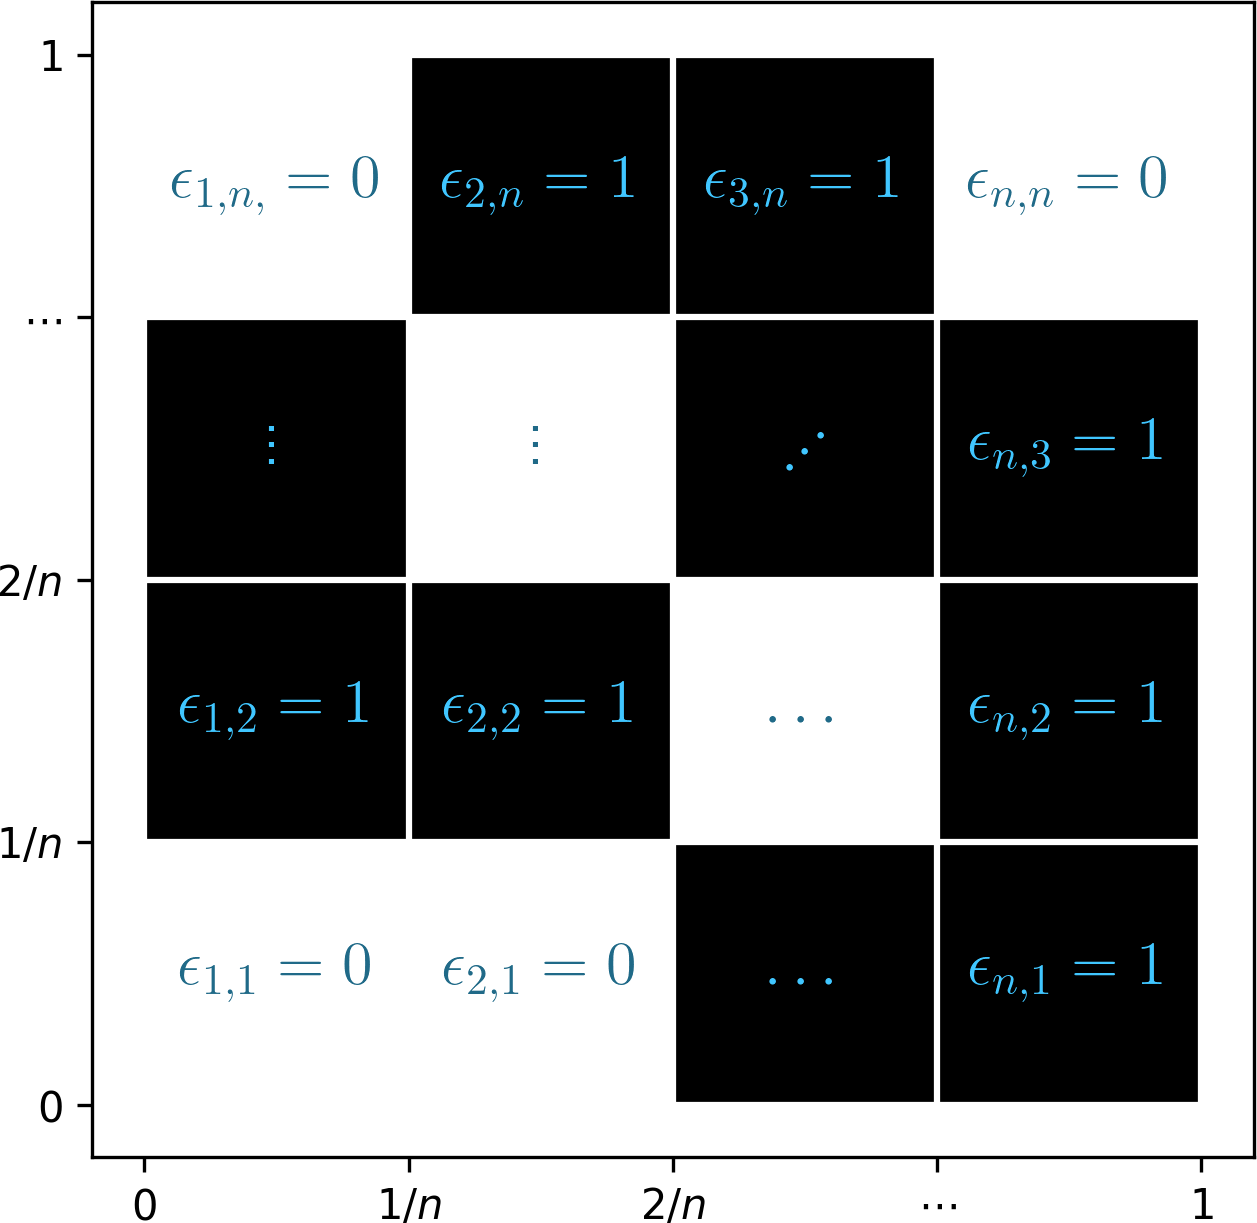
\includegraphics[width=6.5cm]{plain_percolation}
	\caption{Classical Percolation\\($n=4, p=0.6$)}
	\label{fig:classicalPercolation}
\end{wrapfigure}
\subsection{Classical Percolation}
The "classical" percolation is the simplest one, as it is only composed of one filtration.
The formal definition goes as follows:
Split the unit square $\left[ 0,1 \right]^2$ into $n^2$ squares of side $\nicefrac{1}{n}$, indexed by $1 \leq i,j \leq n$:
$$B_{i,j} = \left[ \frac{i-1}{n}, \frac{i}{n} \right] \times \left[ \frac{j-1}{n}, \frac{j}{n} \right].$$
Then, each square will be selected to stay or will be thrown away, according to random variables $\epsilon_{i,j}$ following a Bernoulli distribution with probability parameter $p$
\footnote{Writing $x \sim \mathcal{B}(p)$ for $x$ a random variable following a Bernoulli distribution with parameter $p$, i.e. $\mathbb{P}(x=1)=p$ and $\mathbb{P}(x=0)=1-p$.},
$\epsilon_{i,j} \sim \mathcal{B}(p)$.
Finally, the classical percolation $P$ is
$$P = \bigcup_{i,j \text{ s.t. } \epsilon_{i,j}=1} B_{i,j}.$$
%$$P = \bigcup_{\substack{i,j\\ \epsilon_{i,j}=1}} B_{i,j}.$$

We will adopt the notation $P \sim \text{Perc}(n,p,1)$ for such a setup (a classical percolation of side $n$ and probability parameter $p$).

In this case, it is interesting to study the behaviour as $n \to \infty$, we will write $P \sim \text{Perc}(\infty,p,1)$ for $P = \lim_{n \to \infty} P^n$, $P^n \sim \text{Perc}(n,p,1)$.

\begin{wrapfigure}{r}{7.5cm}
	\vspace{-1.2cm}
	\centering
	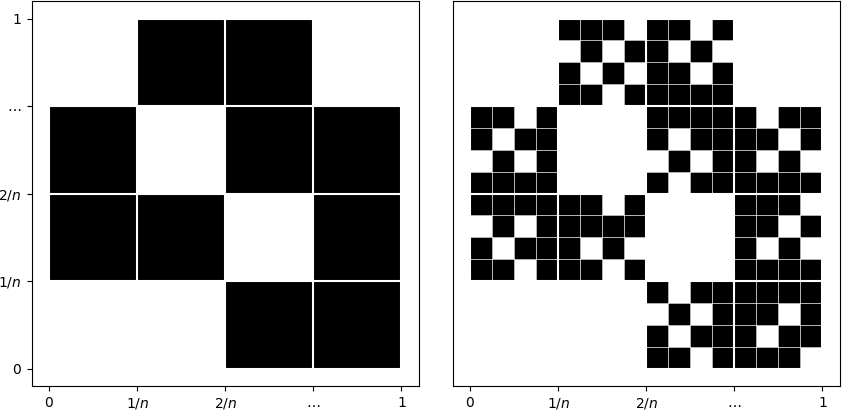
\includegraphics[width=7.5cm]{recursive_percolation_steps}
	\caption{Recursive Percolation\\($n=4, p=0.6, k=1,2$)}
	\label{fig:recursivePercolationSteps}
\end{wrapfigure}
\subsection{Recursive Percolation}
The "recursive" percolation is a little more involved.
Beginning with a classical percolation, we apply an other filtration to each of the remaining squares, and continue recursively.

Formally, for each $1 \leq k \leq d$, split the unit square into $\left( n^k \right)^2$ squares of side $\nicefrac{1}{n^k}$ indexed by $1 \leq i,j \leq n^k$
$$B_{i,j}^k = \left[ \frac{i-1}{n^k},\frac{i}{n^k} \right] \times \left[ \frac{j-1}{n^k},\frac{j}{n^k} \right].$$
Again, associate to each square a Bernoulli random variable with parameter $p$, $\epsilon_{i,j}^k \sim \mathcal{B}(p)$.
Finally, the recursive percolation $P^d$ is defined recursively by:
$$P^k = P^{k-1} \bigcap \left( \bigcup_{i,j \text{ s.t. } \epsilon_{i,j}^k = 1} B_{i,j}^k \right) \quad \forall \, 1 \leq k \leq d$$
%$$P^k = P^{k-1} \bigcap \left( \bigcup_{\substack{i,j\\ \epsilon_{i,j}^k=1}} B_{i,j}^k \right) \quad \forall \, 1 \leq k \leq d$$
and $$P^0 = \left[ 0,1 \right]^2.$$

We will adopt the notation $P^d \sim \text{Perc}(n,p,d)$ for such a setup (a recursive percolation of depth $d$, side $n$ and probability parameter $p$).

In this case, it is interesting to study the behaviour as $d \to \infty$, with $n$ fixed.
We will write $P \sim \text{Perc}(n,p)$ for $P = \bigcap_{k \to \infty} P^k$, with $P^k$ defined recursively as above.

\begin{figure}[!h]
	\centering
	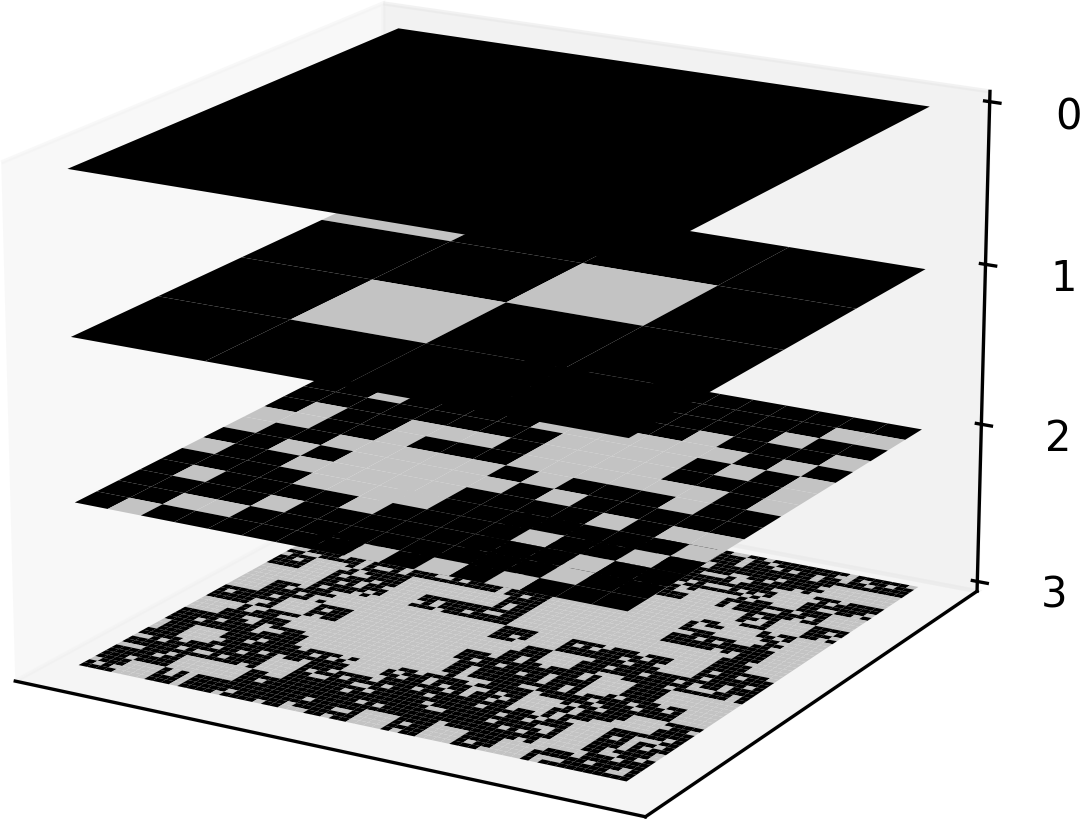
\includegraphics[width=10cm]{recursive_percolation}
	\caption{Recursive Percolation\\($n=4, d=4, p=0.8$)}
	\label{fig:recursivePercolation}
\end{figure}

\subsection{Extension to other dimensions}
Now that we defined percolations in two dimensions, it is straightforward to extend the definition to other dimensions.

\paragraph{Extension to $D$ dimensions}
It suffices to add parameters in the definition to extend it to other dimensions, formally:

\subparagraph{Classical}
Split the unit cuboid $\left[ 0,1 \right]^D$ into $n^D$ squares of side $\nicefrac{1}{n}$, indexed by $1 \leq i_1,\dots,i_D \leq n$:
$$B_{i_1,\dots,i_D} = \left[ \frac{i_1-1}{n}, \frac{i_1}{n} \right] \times \dots \times \left[ \frac{i_D-1}{n}, \frac{i_D}{n} \right].$$
Then, attach to each cuboid a Bernoulli random variable $\epsilon_{i_1,\dots,i_D} \sim \mathcal{B}(p)$.
The classical percolation $P$ in $D$ dimensions is
$$P = \bigcup_{i_1,\dots,i_D \text{ s.t. } \epsilon_{i_1,\dots,i_D}=1} B_{i_1,\dots,i_D}.$$
%$$P = \bigcup_{\substack{i_1,\dots,i_D \\ \epsilon_{i_1,\dots,i_D}=1}} B_{i_1,\dots,i_D}.$$

%The number of remaining squares $Z$ is $Z = | \{ (i_1,\dots,i_D) \mid \epsilon_{i_1,\dots,i_D} = 1 \} |$.
We will denote this setup by $P \sim \text{Perc}^D(n,p,1)$ (a classical percolation of side $n$ and probability parameter $p$ in $D$ dimensions), and write $P \sim \text{Perc}^D(\infty,p,1)$ for $P = \lim_{n \to \infty} P^n$, $P^n \sim \text{Perc}^D(n,p,1)$.

\subparagraph{Recursive}
For each $1 \leq k \leq d$, split the unit cuboid into $\left( n^k \right)^D$ cuboid of side $\nicefrac{1}{n^k}$ indexed by $1 \leq i_1,\dots,i_D \leq n^k$
$$B_{i_1,\dots,i_D}^k = \left[ \frac{i_1-1}{n^k},\frac{i_1}{n^k} \right] \times \dots \times \left[ \frac{i_D-1}{n^k},\frac{i_D}{n^k} \right].$$
Again, attach to each cuboid a Bernoulli random variable $\epsilon_{i_1,\dots,i_D}^k \sim \mathcal{B}(p)$.
Finally, the recursive percolation $P^d$ is defined by:
$$P^k = P^{k-1} \bigcap \left( \bigcup_{i_1,\dots,i_D \text{ s.t. } \epsilon_{i_1,\dots,i_D}^k = 1} B_{i_1,\dots,i_D}^k \right) \quad \forall \, 1 \leq k \leq d$$
%$$P^k = P^{k-1} \bigcap \left( \bigcup_{\substack{i_1,\dots,i_D \\ \epsilon_{i_1,\dots,i_D}^k=1}} B_{i_1,\dots,i_D}^k \right) \quad \forall 1 \leq k \leq d$$

and $$P^0 = \left[ 0,1 \right]^2.$$

We will denote this setup by $P^d \sim \text{Perc}^D(n,p,d)$ (a recursive percolation of depth $d$, side $n$ and probability parameter $p$ in $D$ dimensions).
And again, we will write $P \sim \text{Perc}^D(n,p,\infty)$ for $P  = \bigcap_{k \to \infty} P^k$, with $P^k$ as above.

In practice, we will never use more than three dimensions.
First, because our world is in three dimensions, so it makes sense to stop there.
In addition to that, the curse of dimensionality\cite{WikiDimCurse} stops us (calculations and notations are too heavy from a mathematical point of view, and computations are too expensive from a modelling perspective).


\begin{wrapfigure}{r}{6.5cm}
	\vspace{-0.5cm}
	\centering
	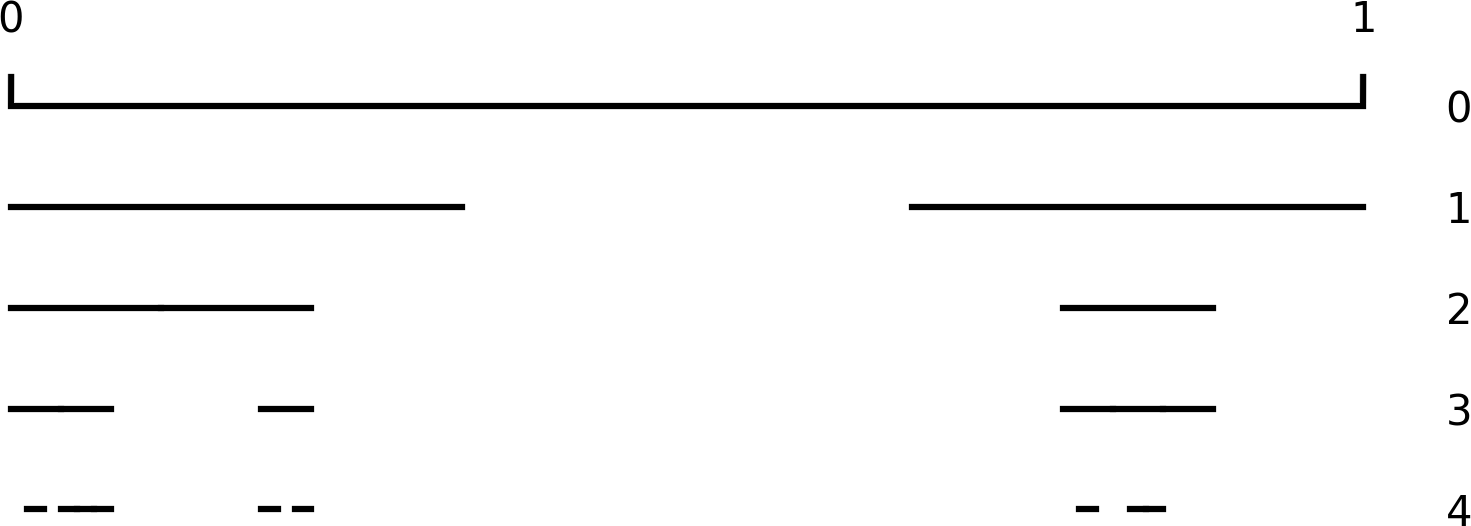
\includegraphics[width=7cm]{Cantor_percolation}
	\caption{1D Recursive Percolation\\($n=3, d=4, p=0.6$)}
	\label{fig:CantorPercolation}
	\vspace{-1cm}
\end{wrapfigure}
\paragraph{Restriction to 1 dimension}
The restriction of the percolation process to one dimension can be thought as a generalized and randomized version of the Cantor set.
The Cantor set splits the interval in 3 equal parts, and keeps the two extreme ones, while the general recursive percolation process splits the interval into $n$ equal parts, and keeps each interval with probability $p$.

\subsection{Density}\label{density}
Since the percolation process involves randomness, the density is not well defined.
However, it is possible to calculate the expected density
\footnote{The density of a set $X \subseteq \left[ 0,1 \right]^D$ is the proportion of points in the unit cuboid that are also in $X$.}.

It is straightforward to remark that the expected density of a classical percolation $P \sim \text{Perc}^D(n,p,1)$ is $p$ (for all $D$ and all $n$).
Note that this density is constant as $n \to \infty$.

Now, for a recursive percolation $P$ such that $P \sim \text{Perc}^D(n,p,d)$, the expected density is $p^d$.
Note that this density tends to zero as $d$ grows to infinity (except in the trivial case $p=1$).
Thus, if $P \sim \text{Perc}^D(n,p,\infty)$, the expected density is $0$.

In two dimensions ($D = 2$), the recursive percolations dimension behave as in fig. \ref{fig:density}.
\begin{figure}[!h]
	\centering
	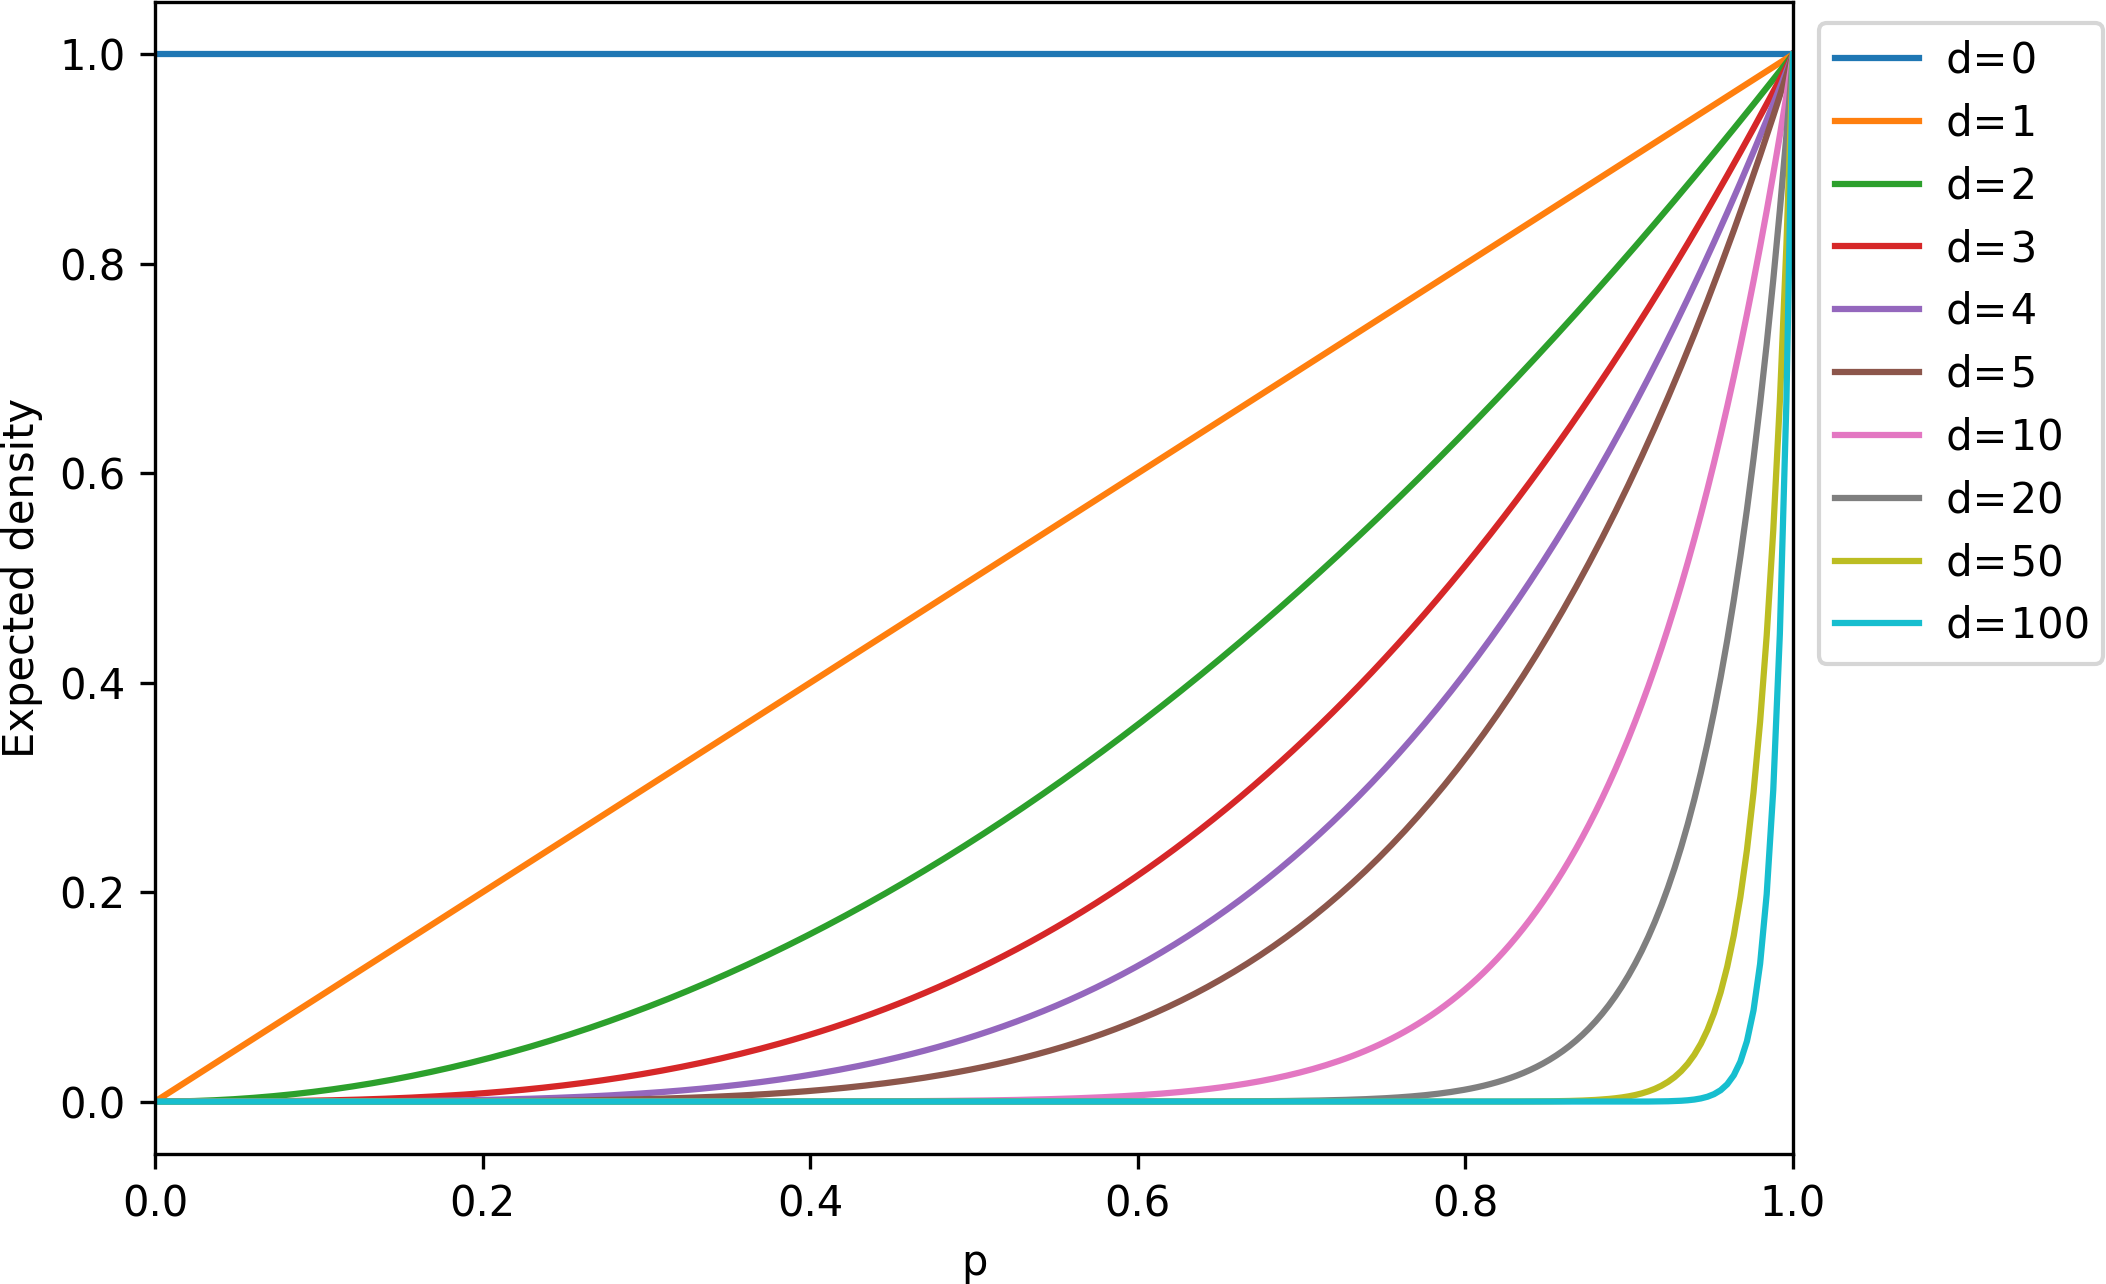
\includegraphics[width=12cm]{density}
	\caption{Density of recursive percolation fractals $P \sim \text{Perc}^2(\infty,p,d)$.}
	\label{fig:density}
\end{figure}

\subsection{Dimensionality}
Again, we can only give an expected dimension, as the process involves randomness.
We ignore the cases $p=0$ and $p=1$ (these are trivial), and we concentrate on $p \in (0,1)$.

We will treat separately the finite case, and the two limit cases (limit as classical percolation, and as recursive percolation).

\paragraph{Finite Case}
Take $n$ and $d$ finite, $P \sim \text{Perc}^D(n,p,d)$.
Let $Z$ be the number of remaining squares ($Z = | \{ (i_1,\dots,i_D) \mid \epsilon_{i_n,\dots,i_D} = 1 \} |$).
%The expected number of remaining squares is then $\mathbb{E}(Z) = \left( p \left( n^D \right) \right)^d$.

There are two possibilities for the dimension of $P$:
\begin{enumerate}
	\item $Z=0$: then $P = \emptyset$ and dimension of $P$ is $0$;
	\item $Z>0$: then $P \supseteq \left[ \frac{i_1-1}{n^k},\frac{i_1}{n^k} \right] \times \dots \times \left[ \frac{i_D-1}{n^k},\frac{i_D}{n^k} \right]$ for some $(i_1,\dots,i_D)$, so dimension of $P$ is $D$.
\end{enumerate}
Therefore, the expected dimension of $P$ is:
$$
\mathbb{E}(\dim_H(P)) = 0.\mathbb{P}(Z=0) + D.\mathbb{P}(Z>0) = D \left( 1 - \left( 1-p\right) ^{\left( n^D \right)^d} \right).
$$
In practice, this is close to $D$, as soon as $n$ or $d$ grows.
Note that $\dim_T$ would only differ by the fact that $\dim_T(\emptyset) = -1$ whereas $\dim_H(\emptyset) = 0$.
Box dimension $\dim_B$ will be the same as the Hausdorff one.

\paragraph{Classical Percolation}
We are looking at $P \sim \text{Perc}^D(\infty,p,1)$.
\subparagraph{Heuristic Argument}
Intuitively, the expected dimension of this percolation should be $D$, since the density is positive.
\subparagraph{Formal Calculations}
We show that the Hausdorff dimension is $D$ almost surely.

Let $\mathcal{U}$ be an open cover for $P$, and let $V$ be an open subset of the unit cuboid of dimension $D$.
Then, $\mathbb{P}(P \cap V = \emptyset) = 0$ (as $V$ is uncountable).
Thus, it is almost sure that $\mathcal{U}$ covers $\left[ 0,1 \right]^D$ (otherwise, there is an open subset $V$ of $\left[ 0,1 \right]^D$ not intersecting $P$).
So $H_{\epsilon}^d(P) = H_{\epsilon}^d\left( \left[ 0,1 \right]^D \right)$ almost surely.
Therefore, $\dim_H(P) = \dim_H(\left[ 0,1 \right]^D) = D$ almost surely.

Note that the almost sure dimension gives the expected dimension.

\paragraph{Recursive Percolation}
We are interested in $P \sim \text{Perc}^D(n,p,\infty)$.

\subparagraph{Eventually Empty Percolation}
In the case of $p < \nicefrac{1}{n^D}$, the number of expected cuboid is less than one.
Thus, as $d \to \infty$, the percolation will almost surely become empty.
Therefore, for $p < \nicefrac{1}{n^D}$, $\dim_H(P) = 0$ almost surely. 

Next, we will suppose $p \geq \nicefrac{1}{n^D}$.

\subparagraph{Heuristically}
In the case of a recursive percolation, $P$ has self-similar properties that can help finding the expected dimension.
After the first percolation, each selected cuboid is another version of $P$ scaled by $\nicefrac{1}{n}$.
This goes on recursively.
Therefore, the intuitive dimension to expect is 
$$\mathbb{E}(\dim_H(P)) = \frac{\ln(\mathbb{E}(Z_1))}{\ln(n)}.$$
Where $Z_1$ is the number of remaining cuboids after one filtration $Z_1 = \left| \{ (i_1,\dots,i_D) \mid \epsilon_{i_n,\dots,i_D}^1 = 1 \} \right|$.
So $\mathbb{E}(Z_1) = p n^D$, and finally:
$$\mathbb{E}(\dim_H(P)) = \frac{\ln(p n^D)}{\ln(n)} = D + \log_n(p).$$

\subparagraph{Formally}
We let the percolation at level $k$ be the union of cuboids/empty sets $C_{i_1,\dots,i_k}$:
$$
P^k = \bigcup_{i_j \in \llbracket 1, \ n^D \rrbracket, 1 \leq j \leq k} C_{i_1,\dots,i_k}
$$
where $C_{i_1,\dots,i_k}$ is the $i_k^{th}$ sub-cuboid of $C_{i_1,\dots,i_{k-1}}$ if it has been selected by the random process, and the empty set otherwise.
When $C_{i_1,\dots,i_k}$ is non-empty, we let 
\begin{equation*}
	R_{i_1,\dots,i_k} =
	\begin{cases}
		\frac{1}{n} \footnotemark & \text{if } \  C_{i_1,\dots,i_k} \neq \emptyset \\
		0 & \text{else (i.e. if } \  C_{i_1,\dots,i_k} = \emptyset \text{ )}
	\end{cases}
\end{equation*}
\footnotetext{Note that $\frac{1}{n}$ is the scaling ratio from $C_{i_1,\dots,i_{k-1}}$ to $C_{i_1,\dots,i_k}$ (when not empty).}
%$$ R_{i_1,\dots,i_k} = \frac{\| C_{i_1,\dots,i_k \|}}{\| C_{i_1,\dots,i_{k}-1 \|}}. $$
We take $\Omega$ to be our sample space, and assume that a probability measure $\mathbb{P}$ is defined on a suitably large family $\mathcal{F}$ of subsets of $\Omega$, such that the ratios $R_{i_1,\dots,i_k}$ are random variables.
By the self-similarity of the percolation construction, all the $R_{i_1,\dots,i_k}$ have the same distribution.

We write $\mathbb{E}\left( X \mid \mathcal{F}_k \right)$ for the conditional expectation of a random variable $X$ given the knowledge of $R_{i_1,\dots,i_j}$ for all sequences $i_1,\dots,i_j$ such that $j \leq k$.

Using this setup and following the same steps as in \cite[p268-271, proof of Th. 15.1]{Falconer_1990}\footnote{Calculating $\mathbb{E}\left( \sum_{R \in P^k} \| R \|^s \right)$ and using $\mu(R) = \lim_{j \to \infty} \left\{ \sum \|\tilde{R}\|^s \mid \tilde{R} \in R_j \text{ and } \tilde{R} \subseteq R \right\}$, with $\| S \|$ the $D$ dimensional Lebesgue measure of the set $S$ (all our set being in $\R^D$).} we have that with probability one\footnote{Remember we are in the case $p>\frac{1}{n^D}$.}, $\dim_H(P) = s$ with $s$ the solution of the expectation equation
$$\mathbb{E}\left( \sum_{i=1}^{n^D} R_i^s \right) = 1.$$
that is, 
$$n^Dp\frac{1}{n^s} = 1 \iff s = D + \log_n(p).$$
Therefore, the almost sure dimension of $P$ is $\dim_H(P) = D + \log_n(p)$.

This idea is generalised in \cite[p.271, Th. 15.2]{Falconer_1990}.

%%% WRONG PROOF:
%If no randomness is involved in the process, the above argument can be made rigorous:
%Define a contractive map that reflects the self similarities.
%Then use Stefan Banach's contractive mapping fixed point theorem applied to the complete metric space of non-empty compact subsets of $R^n$ with the Hausdorff distance.
%
%We show the fractional dimension is $\alpha = D + \log_n(p)$ directly (this proof follows some ideas from \cite[p. 265-273, section 15]{Falconer_1990}).
%
%From definition, $P = \bigcap_{d \to \infty} P^k$.
%$P^k$ is composed of cuboids of side $\nicefrac{1}{n^k}$.
%Let $Z^k$ be the number of these cuboids.
%%(i.e. $Z^k = \left| \{ (i_1,\dots,i_D) \mid \epsilon_{i_n//n^{k-j},\dots,i_D//n^{k-j}}^j = 1 \quad \forall j \leq k \} \right|$.
%In expectation, $P^k$ should have $\mathbb{E}(Z^k) = \left( p n^D \right)^k$ cuboids of side $\nicefrac{1}{n^k}$ remaining.
%Taking $P^k$ as a $\beta_k$-cover of $P$, with $\beta_k = \nicefrac{\sqrt{D}}{n^k}$
%\footnote{So that $\beta_k$ is the diameter of a cuboid of side $\nicefrac{1}{n^d}$ in dimension $D$.}, we have
%$$\mathbb{E}\left( H_{\beta_k}^{\alpha}(P) \right) \leq \left( p n^D \right)^k \left( \nicefrac{\sqrt{D}}{n^k} \right)^{D + \log_n(p)} \leq \sqrt{D}^{\alpha}.$$
%Letting $k \to \infty$, we get
%$$\mathbb{E} \left( H^{\alpha}(P) \right) \leq \sqrt{D}^{\alpha} < \infty.$$

%Now, we show that $\mathbb{E} \left( H^{\alpha}(P) \right)  > 0$:
%Let $\mathcal{U} = \{ U_i \mid i \in I \}$ be an open cover of $P$.
%For each $i \in I$, let $k \in \N$ be such that $\beta_{k+1} \leq \diam{U_i} < \beta_k$.
%Then, in general, $U_i$ may only cover fully one cuboid from $P^k$.
%%As generating $P$ is a random process, it may happen that a $U_i$ covers more than one, but this is not the case in general (as it involves a very particular selection configuration), and will not be consistently the case as we take $k \to \infty$.
%Now, if $j \geq k$, then $U_i$ intersects in expectation at most $\left( p n^D \right)^{j-k}$ cuboids of side $\nicefrac{1}{n^j}$ (note $\left( p n^D \right)^{j-k} \leq \frac{\left( pn^D \right)^j}{\sqrt{D}^{\alpha}} \diam{U_i}^{\alpha}$).
%Taking $j$ such that $\beta_{j+1} \leq \diam{U_i} \quad \text{ for } i \in I$, since $\mathcal{U}$ intersects in expectation $\mathbb{E}(Z^j) = \left( p n^D \right)^j$ cuboids of diameter $\nicefrac{1}{n^j}$, we get
%$$\left( p n^D \right)^j \leq \sum_{i \in I} \frac{\left( pn^D \right)^j}{\sqrt{D}^{\alpha}} \diam{U_i}^{\alpha}.$$
%This implies that in expectation, $\sqrt{D}^{\alpha} \leq H^{\alpha}(P)$.
%Thus, $\mathbb{E} \left( H^{\alpha}(P) \right)  \geq \sqrt{D}^{\alpha} > 0$.
%
%Finally, as $0 < H^{\alpha}(P) < \infty$, we get $\mathbb{E}(\dim_H(P)) = \alpha = D + \log_n(p)$.

\subparagraph{Dimension Plots}
In starting from two dimensions ($D = 2$), the recursive percolations dimension behave as in fig. \ref{fig:dimension2D}.
For plots of $D = 1,\dots,5$ see \url{https://pauldubois98.github.io/PercolationFractalsStudy/percolation.html}.
\begin{figure}[!h]
	\centering
	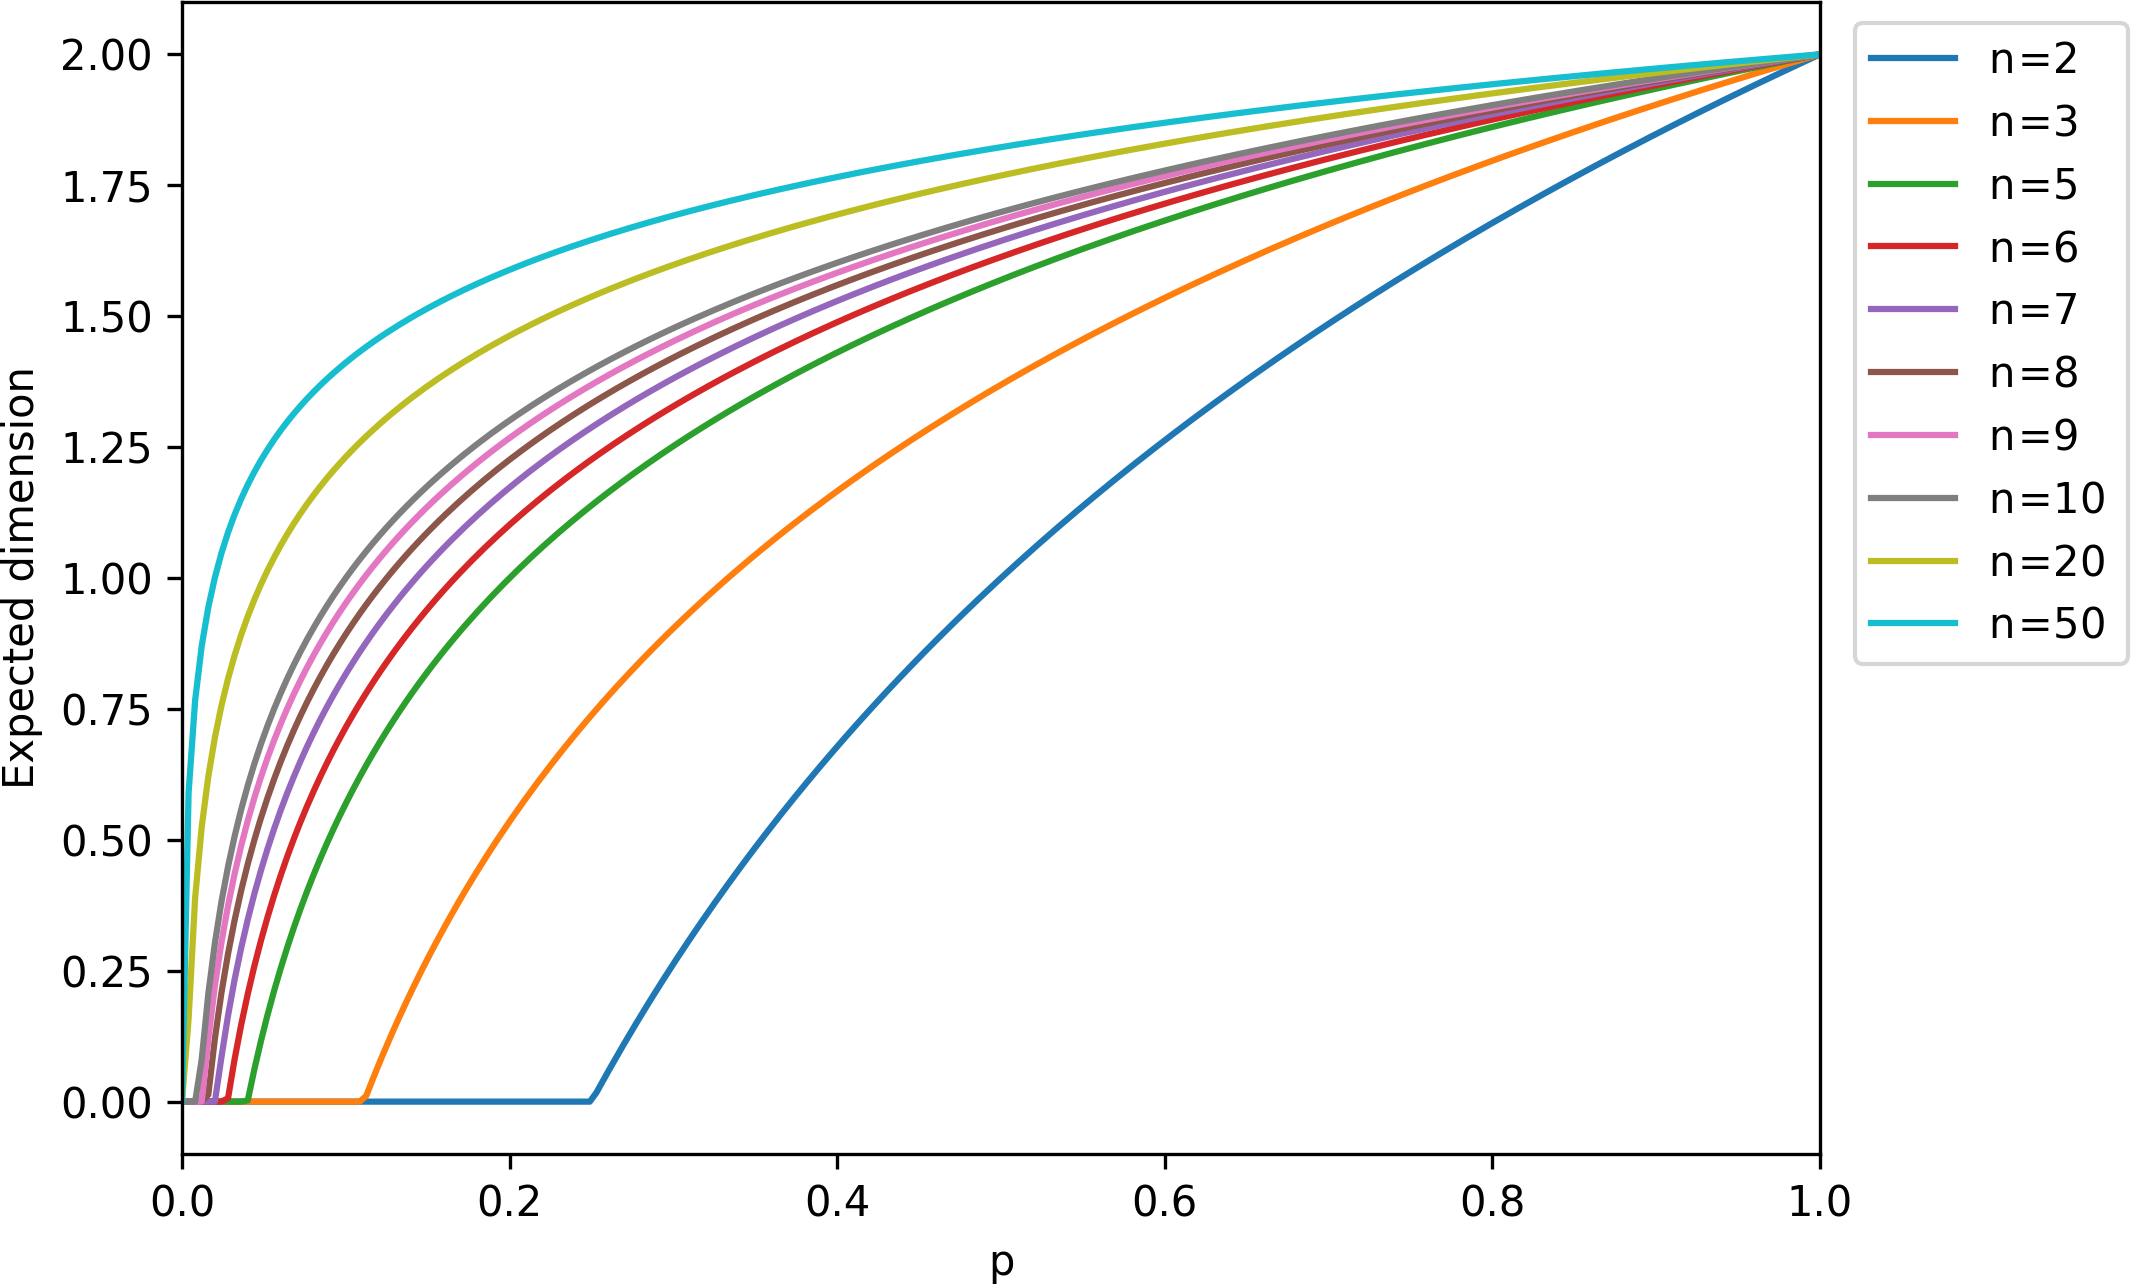
\includegraphics[width=12cm]{dimension_2D}
	\caption{Dimension of recursive percolation fractals $P \sim \text{Perc}^2(n,p,\infty)$.}
	%\caption{Dimension of recursive percolation fractals.}
	\label{fig:dimension2D}
\end{figure}

\subsection{Blob}
To have a better understanding, we begin by studying the central "blob" of the fractal.
\paragraph{Definition}
We define the blob of a percolation $P$ as the connected component of $P$ that contains the point at the center of the cuboid (that is, the component that contains $(\nicefrac{1}{2}, \dots, \nicefrac{1}{2})$).
Note that the blob may be empty.

In the simulations, since infinite percolation may only be approximated, we only consider cases where $n$ is odd, so that the cuboid containing the point $(\nicefrac{1}{2}, \dots, \nicefrac{1}{2})$ is unique.

\paragraph{Algorithm}
The algorithm we use to find the blob is similar to the one used for finding crossings, and will be discussed in details in \ref{crossingAlgorithm}.

We will use four metrics for evaluating the size and regularity of the blob.
\begin{itemize}
	\item The size of the interior of the blob (we will use the $D$-dimensional Lebesgue measure).
	\item The size of the boundary of the blob (we will use the $(D-1)$-dimensional Lebesgue measure).
	\item The maximum (Euclidean) distance from the center (the point $(\nicefrac{1}{2},\dots,\nicefrac{1}{2})$) to the boundary of the blob.
	\item The maximum step distance from the central cuboid (the cuboid containing $(\nicefrac{1}{2},\dots,\nicefrac{1}{2})$) to cuboids at the boundary of the blob. The step distance from a cuboid $A$ to another cuboid $B$ is the minimal length of a cuboid-path linking $A$ and $B$ using only cuboids in the blob.
\end{itemize}
The interior and Euclidean distance measure how large the blob is, while the step distance and the area measure the irregularity.
Figure \ref{fig:blobMeasures} shows the four metrics on a typical percolation blob.

\begin{figure}[!h]
	\centering
	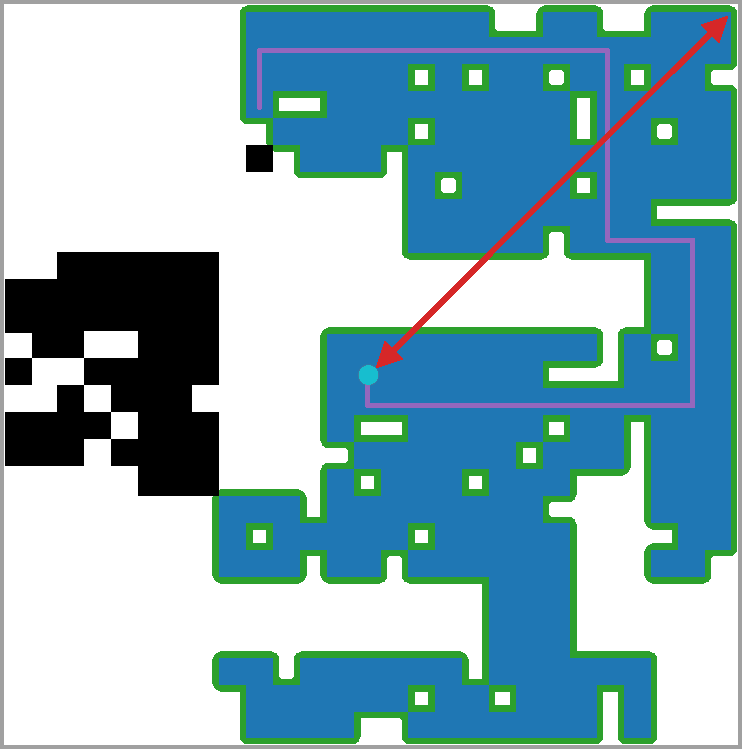
\includegraphics[height=8cm]{blob}
	\caption{Blob Measures:\\
		\textit{Blue:} Blob interior.\\
		\textit{Green:} Blob boundary.\\
		\textit{Red:} Maximum center-boundary Euclidean distance.\\
		\textit{Purple:} Maximum center-boundary step distance.\\
		\textit{Cyan:} Central point $(\nicefrac{1}{2},\dots,\nicefrac{1}{2})$.}
	\label{fig:blobMeasures}
\end{figure}

\paragraph{Simulations}\label{blob}
The study of the central blob from a mathematical theory perspective is hard.
However, it is possible to get some understanding of the blob by generating percolation simulations.
The following results were obtained from taking the average over 50000 percolations generated randomly, and looking at the blob of each percolation.
The approximation is therefore very accurate.
This was possible thanks to Oxford Mathematical Institute's Computing Services.

All plots from our simulations are available at \url{https://pauldubois98.github.io/PercolationFractalsStudy/blob.html}.
They are all of the following form: the probability parameter $p$ on the x-axis, the quantity we are looking at on the y-axis, and a line for each pair of parameters $(n,d)$, labelled with $n \hat{} d$.
We considered the cases $D=2$ and $D=3$.
For $D=2$, the interior is measured by an area, and the boundary by a length, while for $D=3$, the interior is a volume, and the boundary an area.
We will only comment and show here the results for $D=2$, there is not much changes for $D=3$.

\subparagraph{Interior}
For classical percolation (see fig. \ref{fig:blobInteriorClassical}), as $n \to \infty$, there seems to be a jump value around $p=0.6$: for $p<0.6$, the interior is empty, while for $p \geq 0.6$, it is non-empty and the size increase until reaching one for $p=1$.

For recursive percolations (see fig. \ref{fig:blobInteriorRecursive}), we observed the same phenomenon, with a shift to the right (i.e. towards $p=1$) when $d$ increases.
For $d=2$, the jump as $n \to \infty$ seems to occur at $p \approx 0.65$.
When $d \to \infty$, it looks like the area of the blob tends to zero when $p<1$.

In fact, this can be proved: we have shown (back in section \ref{density}) that the density of the percolation in this case tends to zero.
Thus, the area of the percolation $P$ tends to zero.
Since the blob is a subset of $P$, its area must also tend to zero.

\begin{figure}[!h]
	\centering
	\begin{subfigure}{.49\textwidth}
		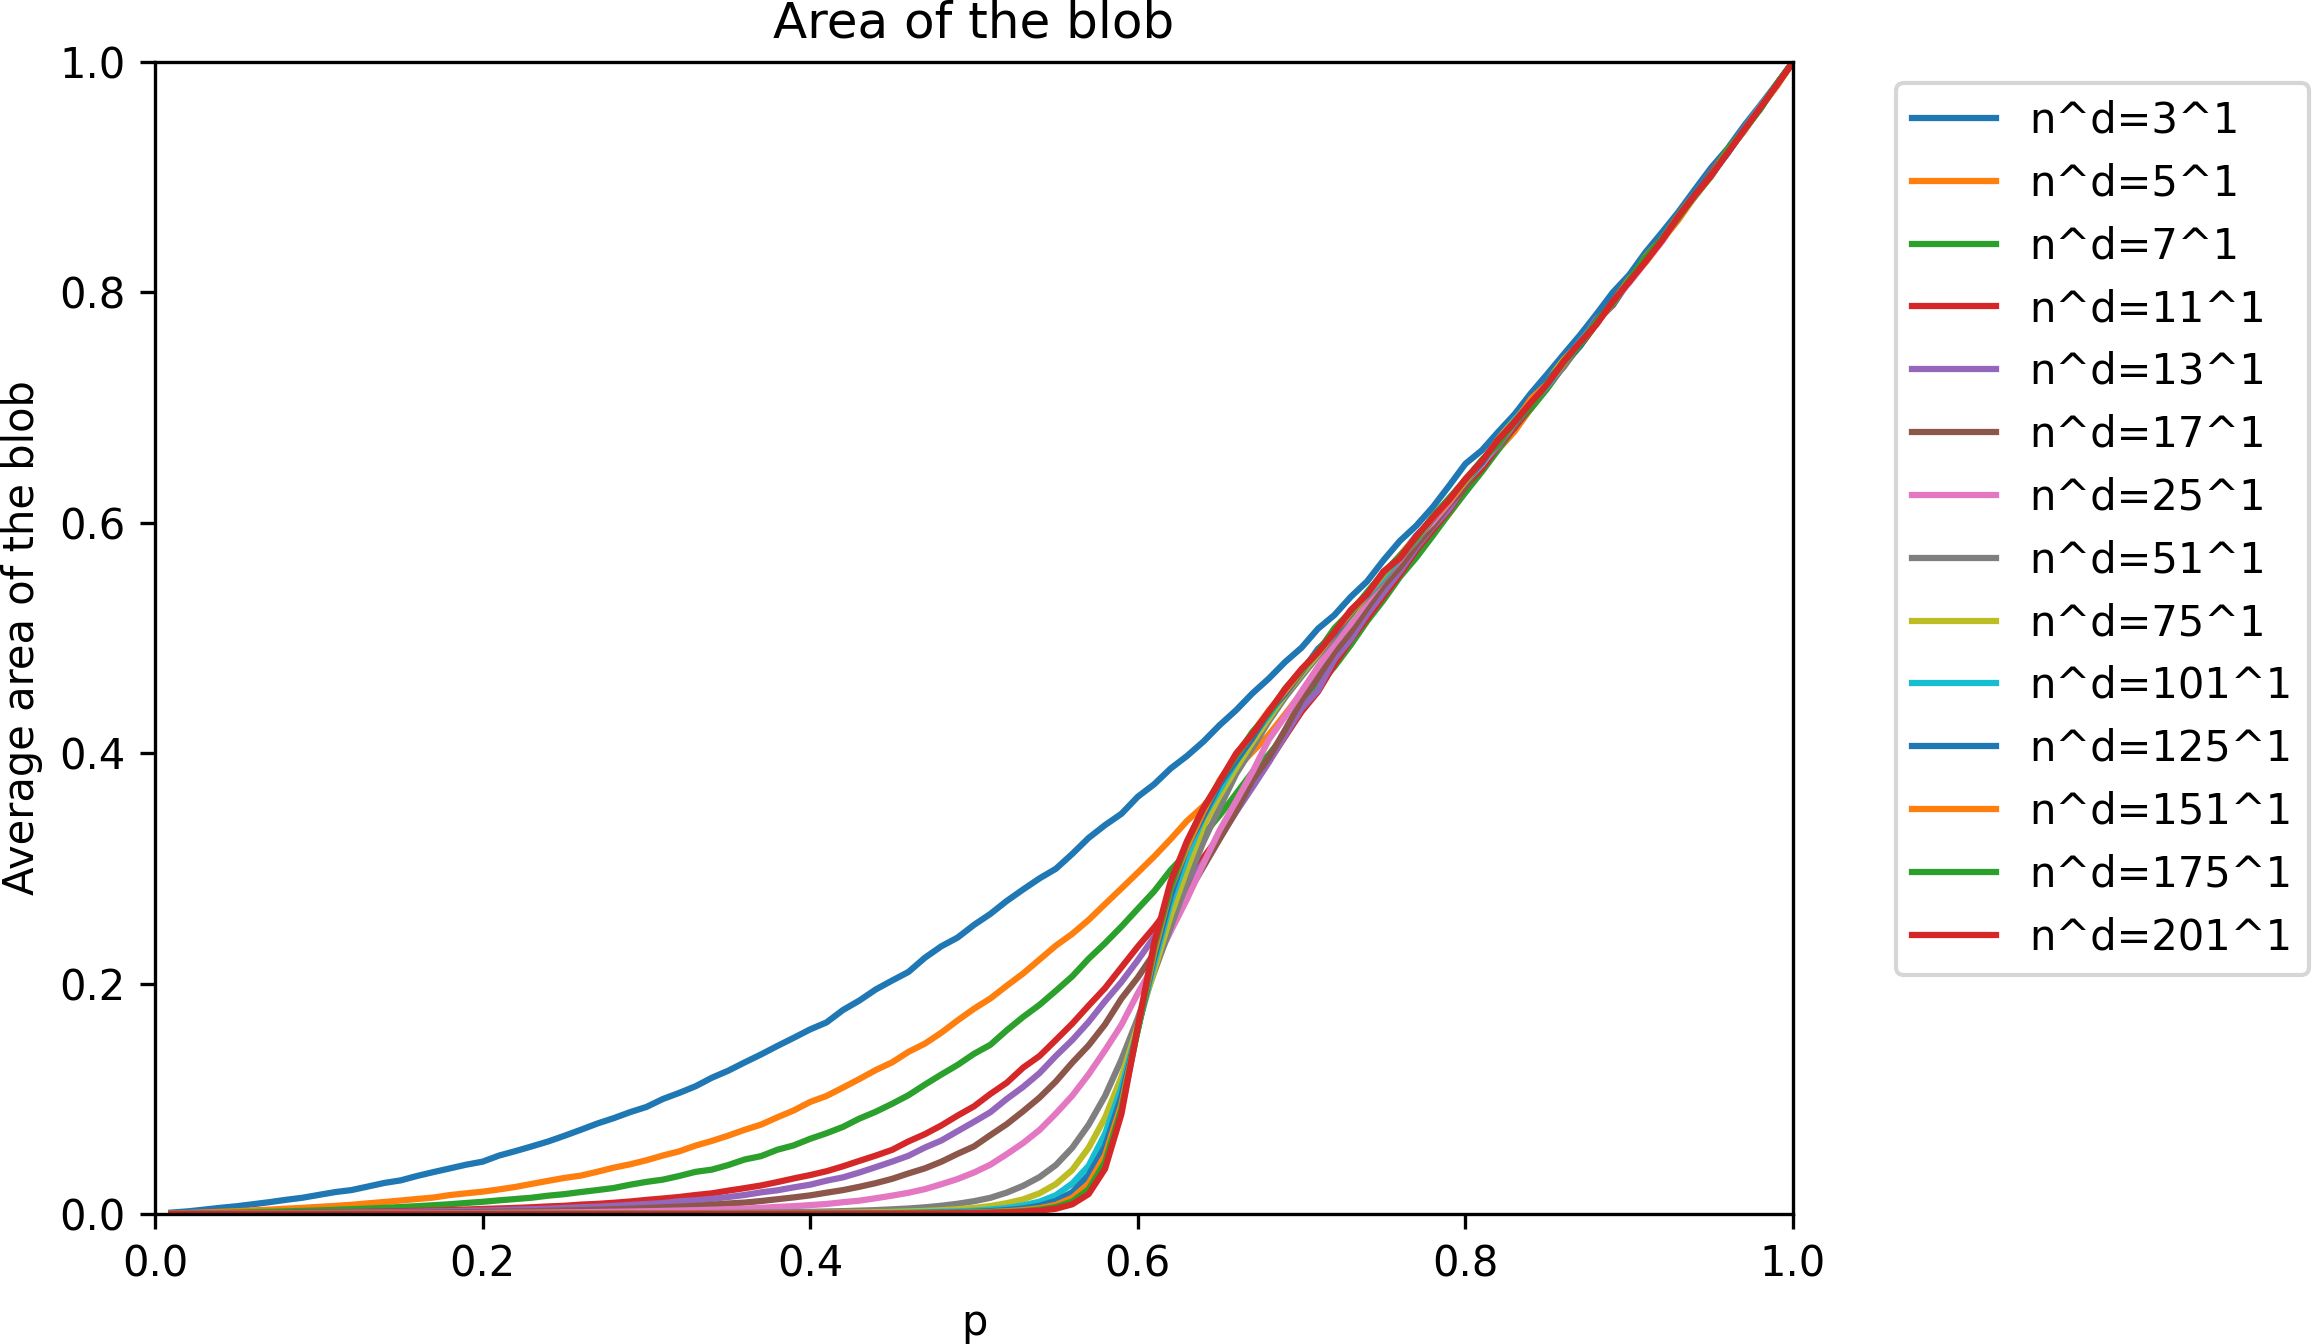
\includegraphics[width=8cm]{blob_interior_2D_classical}
		\centering
		\caption{Classical Percolation}
		\label{fig:blobInteriorClassical}
	\end{subfigure}
	\begin{subfigure}{.49\textwidth}
		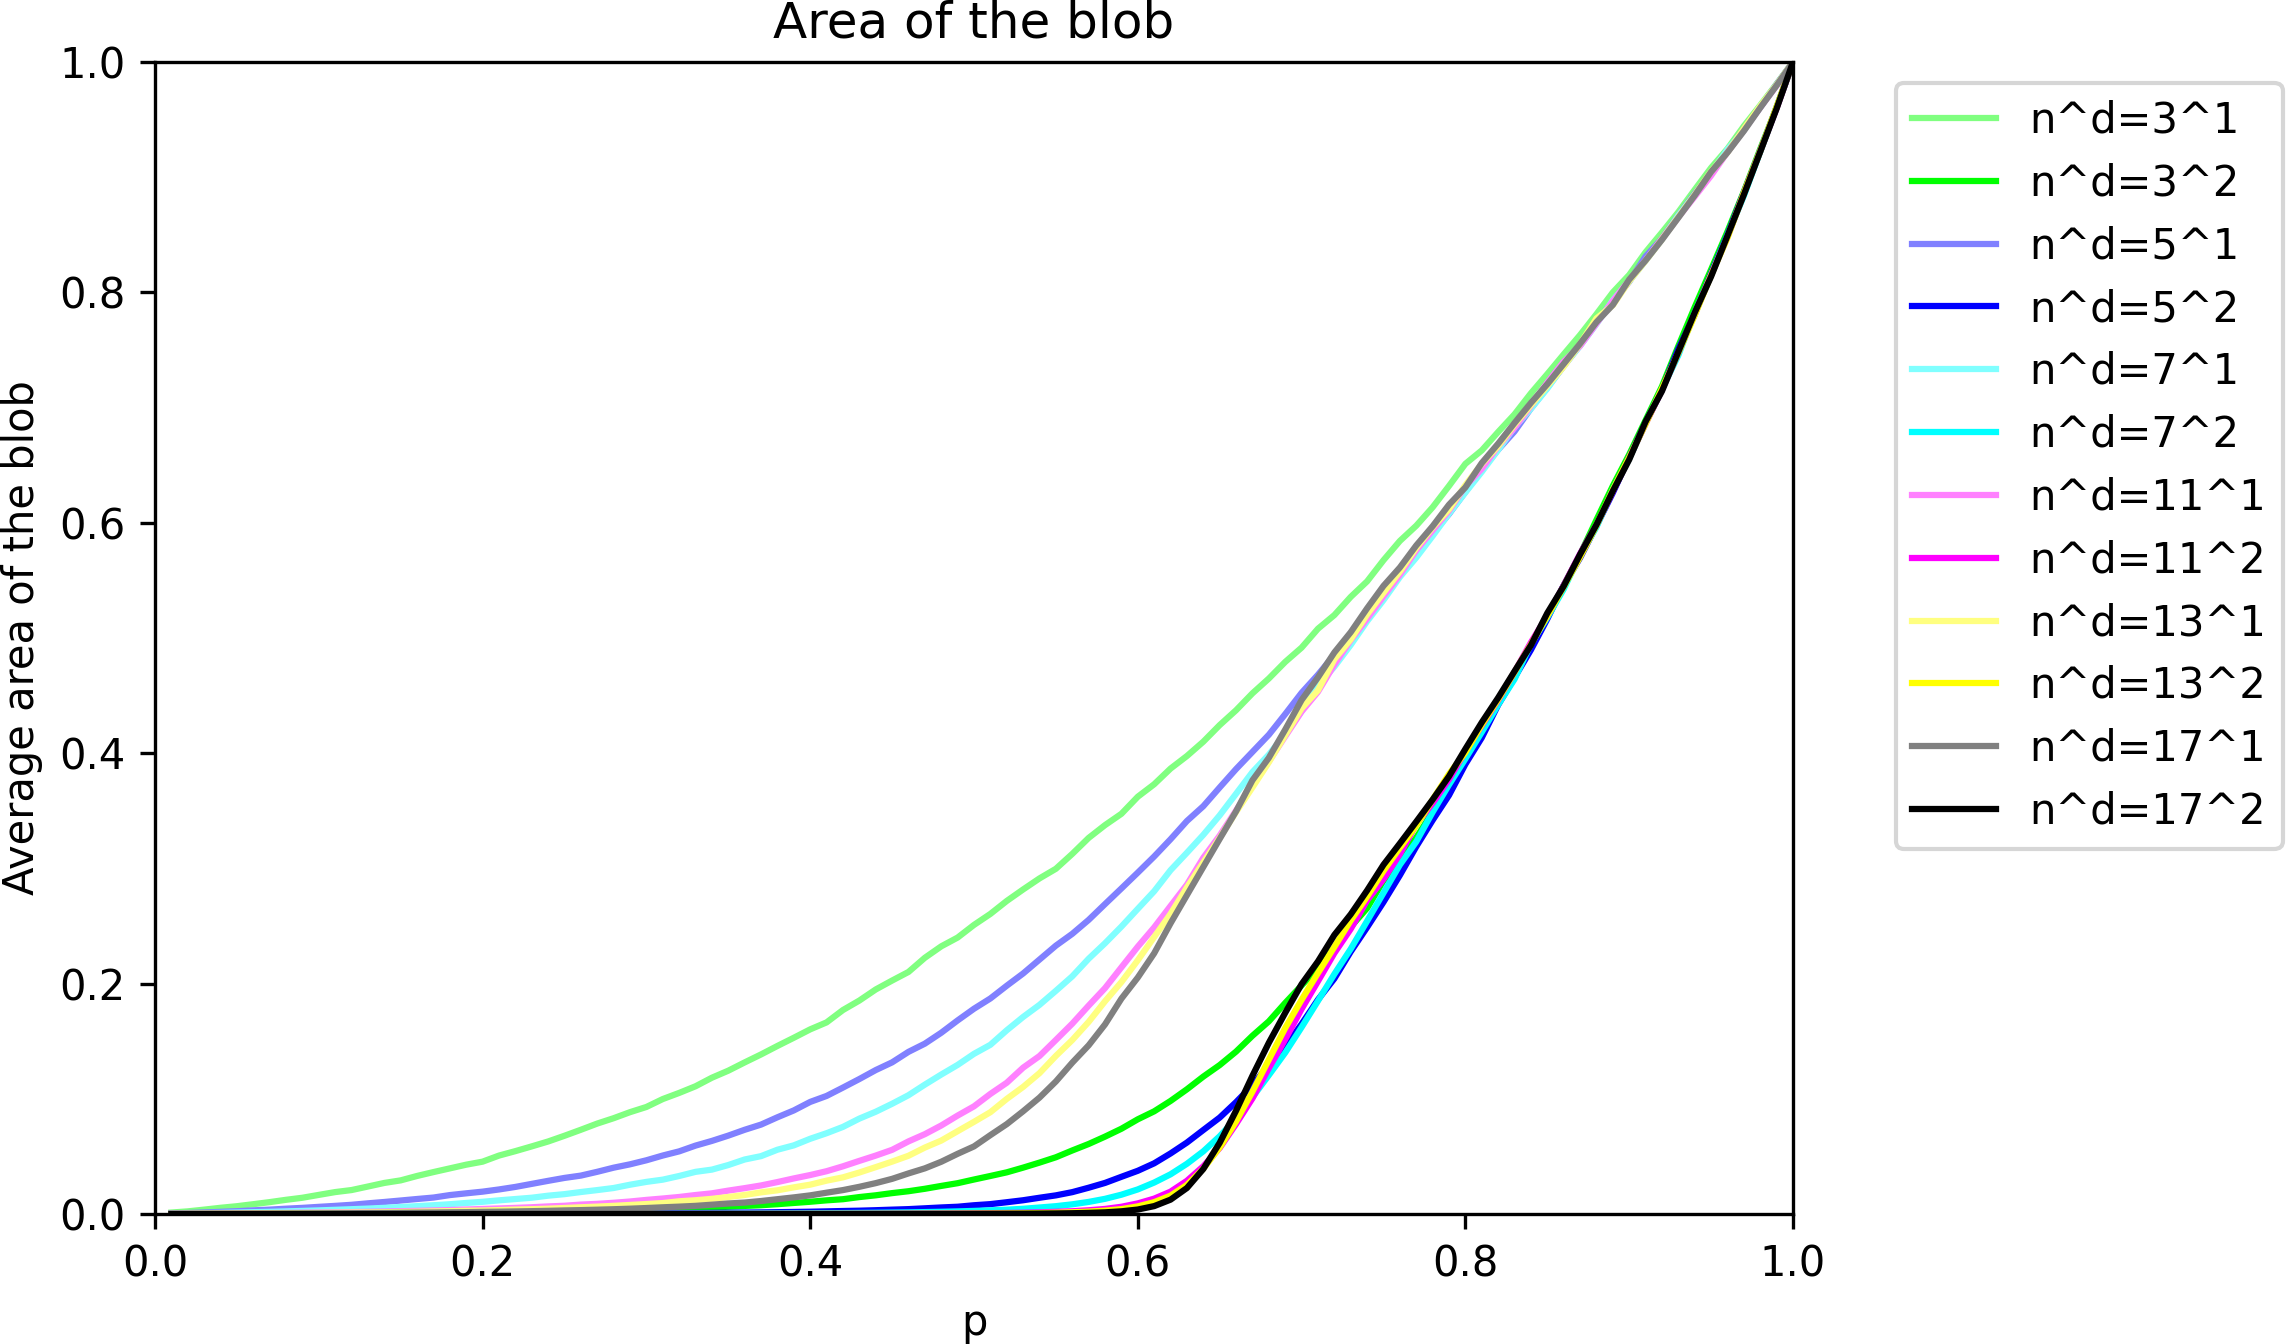
\includegraphics[width=8cm]{blob_interior_2D_recursive_bis}
		\centering
		\caption{Recursive Percolation}
		\label{fig:blobInteriorRecursive}
	\end{subfigure}
	\caption{Blob Interior}
	\label{fig:blobInterior}
\end{figure}


\subparagraph{Euclidean distance center-border}
The Euclidean distance from the central point to the border of the blob is also a measure of the size of the blob.
Therefore, it makes sense that the Euclidean distance (plotted on fig. \ref{fig:blobEuclideanDistance}) and the interior of the blob (fig.\ref{fig:blobInterior}) behave similarly.

\begin{figure}[!h]
	\centering
	\begin{subfigure}{.49\textwidth}
		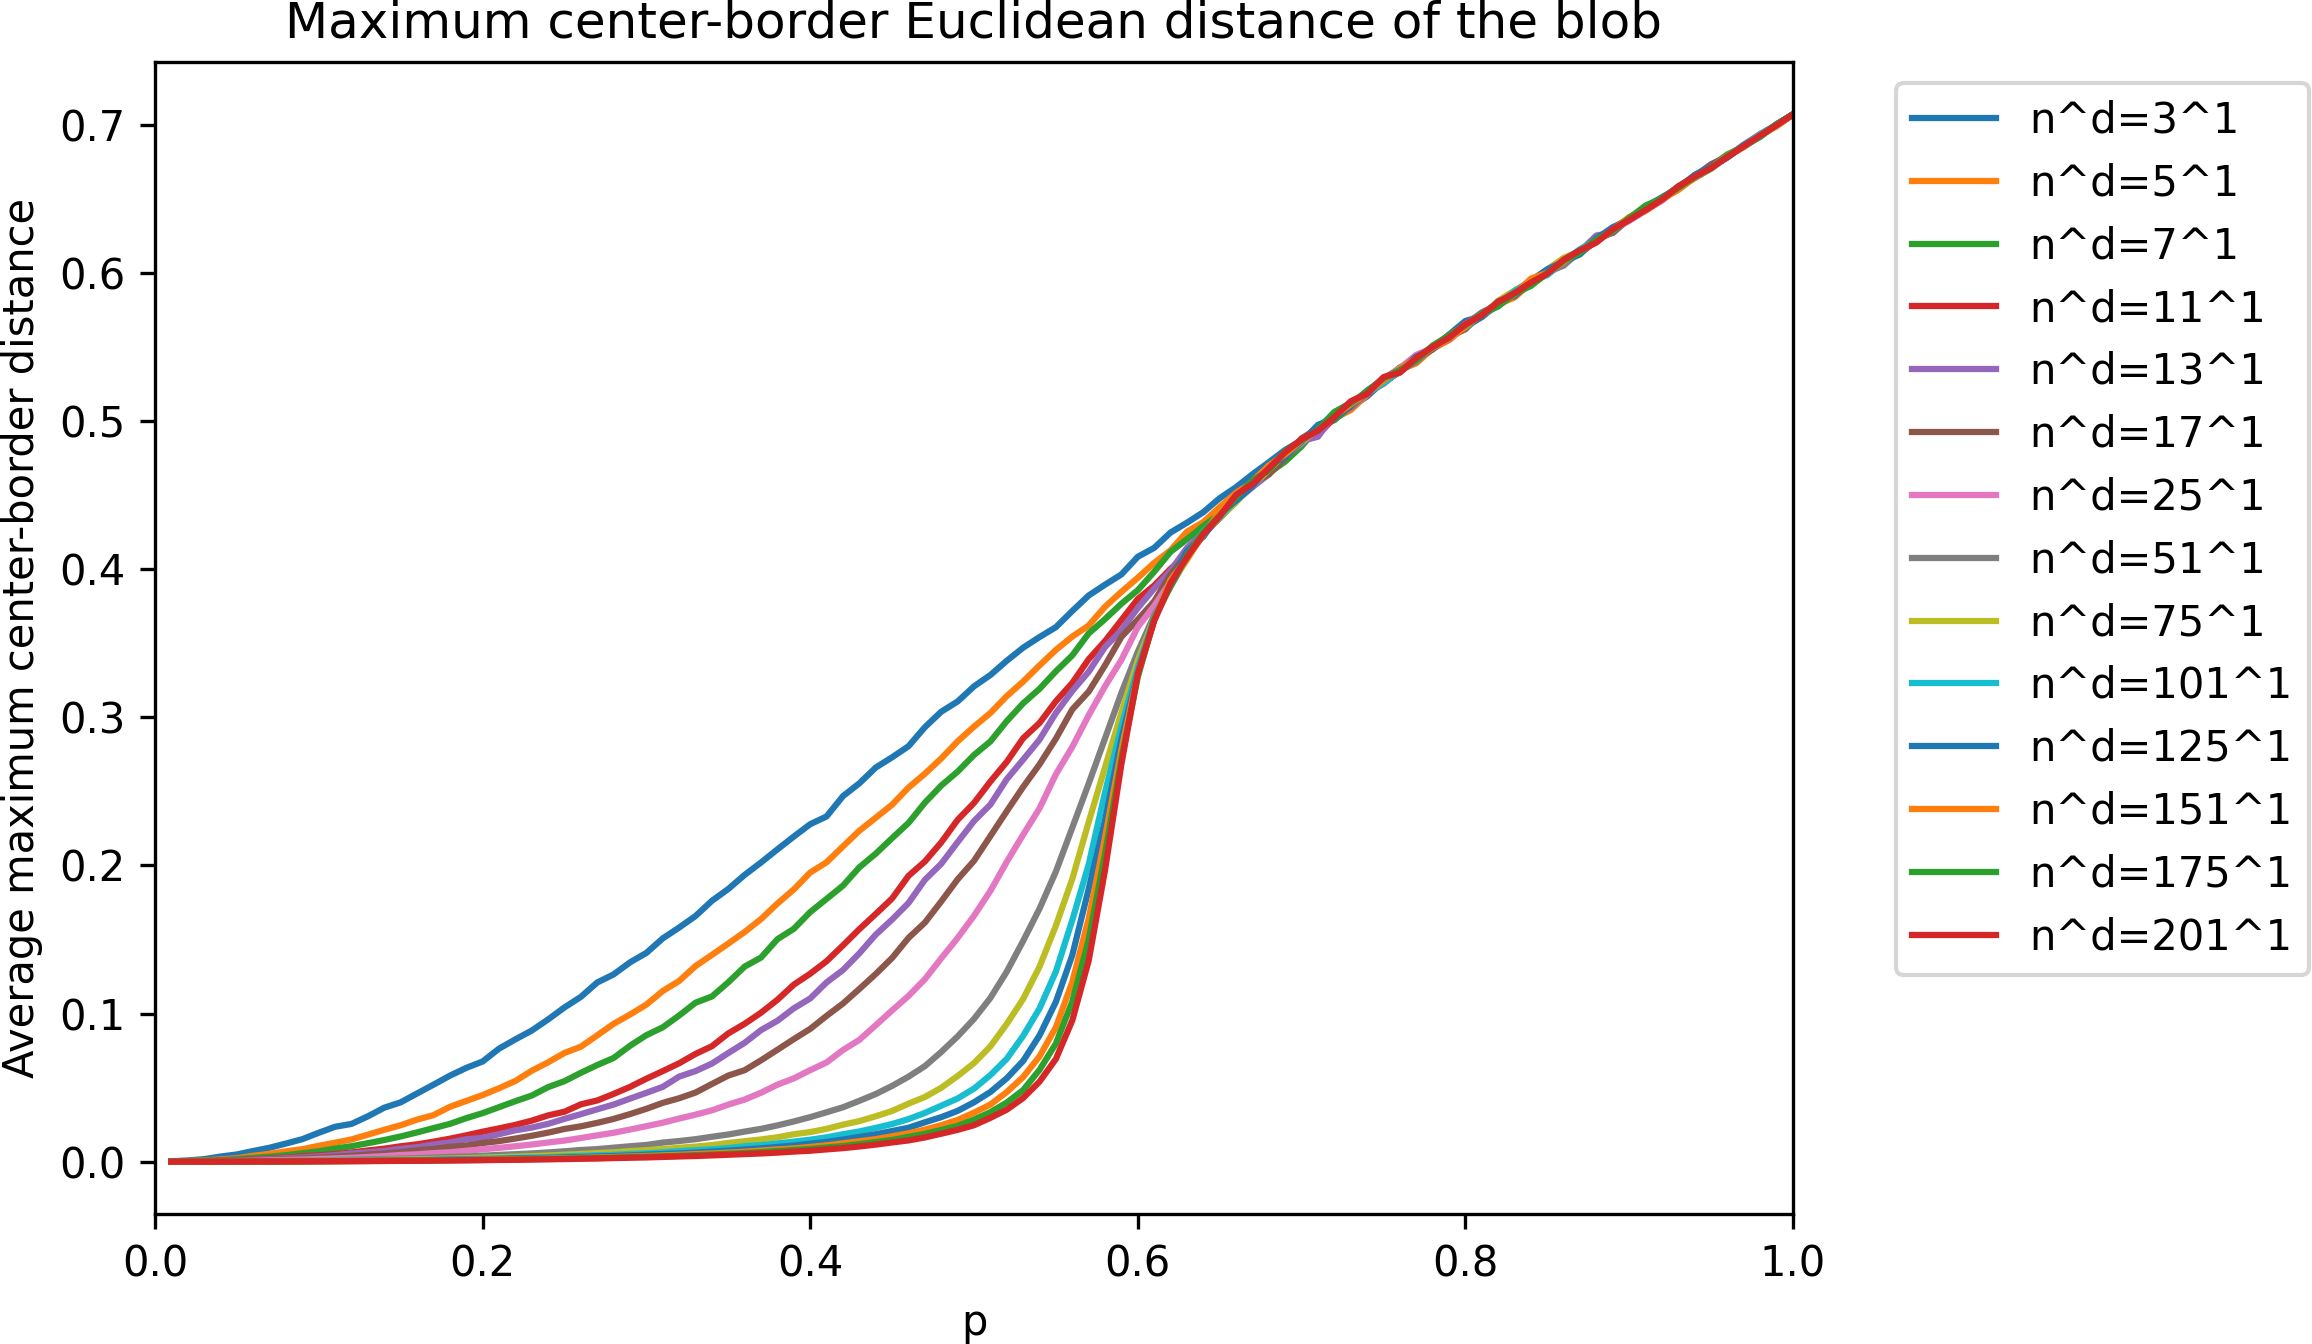
\includegraphics[width=8cm]{blob_dist_2D_classical}
		\centering
		\caption{Classical Percolation}
		\label{fig:blobEuclideanDistanceClassical}
	\end{subfigure}
	\begin{subfigure}{.49\textwidth}
		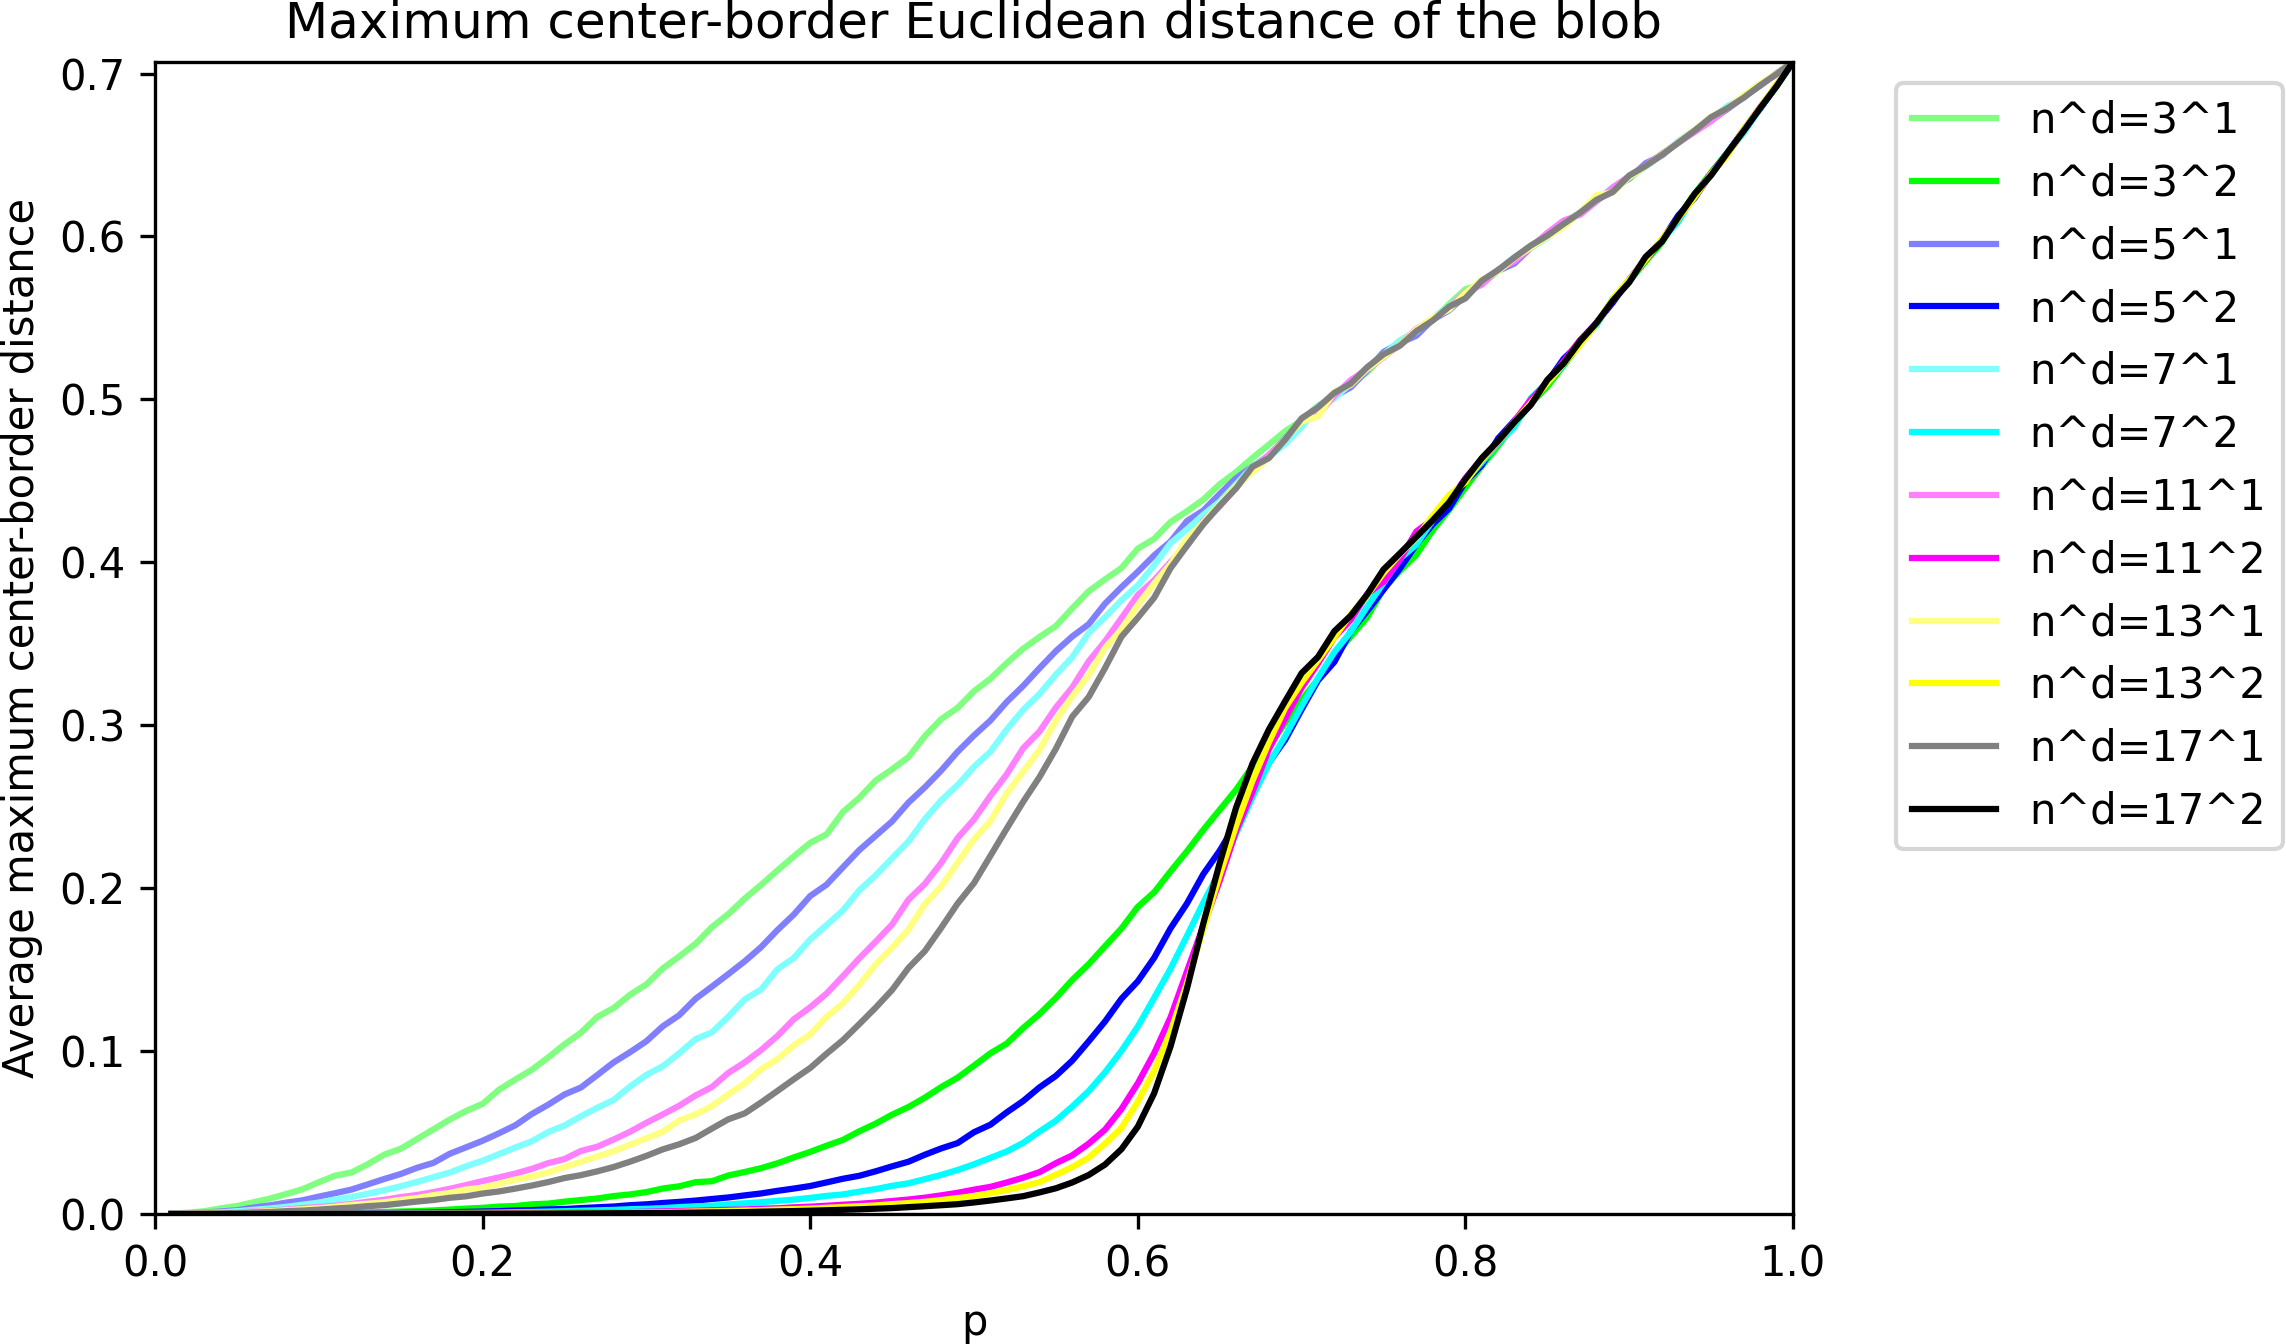
\includegraphics[width=8cm]{blob_dist_2D_recursive_bis}
		\centering
		\caption{Recursive Percolation}
		\label{fig:blobEuclideanDistanceRecursive}
	\end{subfigure}
	\caption{Blob Euclidean Distance}
	\label{fig:blobEuclideanDistance}
\end{figure}


\subparagraph{Boundary}
The size of the boundary of the blob measures how irregular the blob is.
This follows the same idea as when we measure the length of islands coastlines to give a sense on how irregular the islands boundaries are (see \ref{appendix:coastlines}).

For regular ($d=1$) percolations, we observe that when $p<0.6$, the boundary length of the blob is close to zero, together with the fact that the interior area is also close to zero, this yields that the blob is nearly empty on most of the simulations.
We then see a jump behaviour: for $0.6 \leq p <1$, the length of the boundary grows rapidly as $n$ increases.

When $p$ is close to one, the percolation is connected.
The blob and the percolation are nearly the same sets, and the removed cuboids can be assumed to be isolated.
Then, the size of the boundary for $P \sim \text{Perc}^D(n,p,1)$ is (in expectation):
$$\underbrace{(1-p)n^D}_{\text{Expected number of\\cuboids removed}} \underbrace{2D \left( \nicefrac{1}{n} \right)^{D-1}}_{\text{Boundary of a single\\cuboid of side } \nicefrac{1}{n}}
+ \overbrace{2D}_{\text{Boundary of the\\unit cuboid}} = 2D (1 + (1-p)n) \to \infty \quad \text{ as } n \to \infty$$
This behaviour is observed for $D=2$ in \ref{fig:blobBoundaryClassical}.

For recursive percolation (see fig. \ref{fig:blobBoundaryRecursive}), we also observe two phases (boundary close to zero for small $p$, followed by a rapid increase when $p$ gets closer to one).
The probability at which the behaviour split is however different, and increases as $d \to \infty$.

\begin{figure}[!h]
	\centering
	\begin{subfigure}{.49\textwidth}
		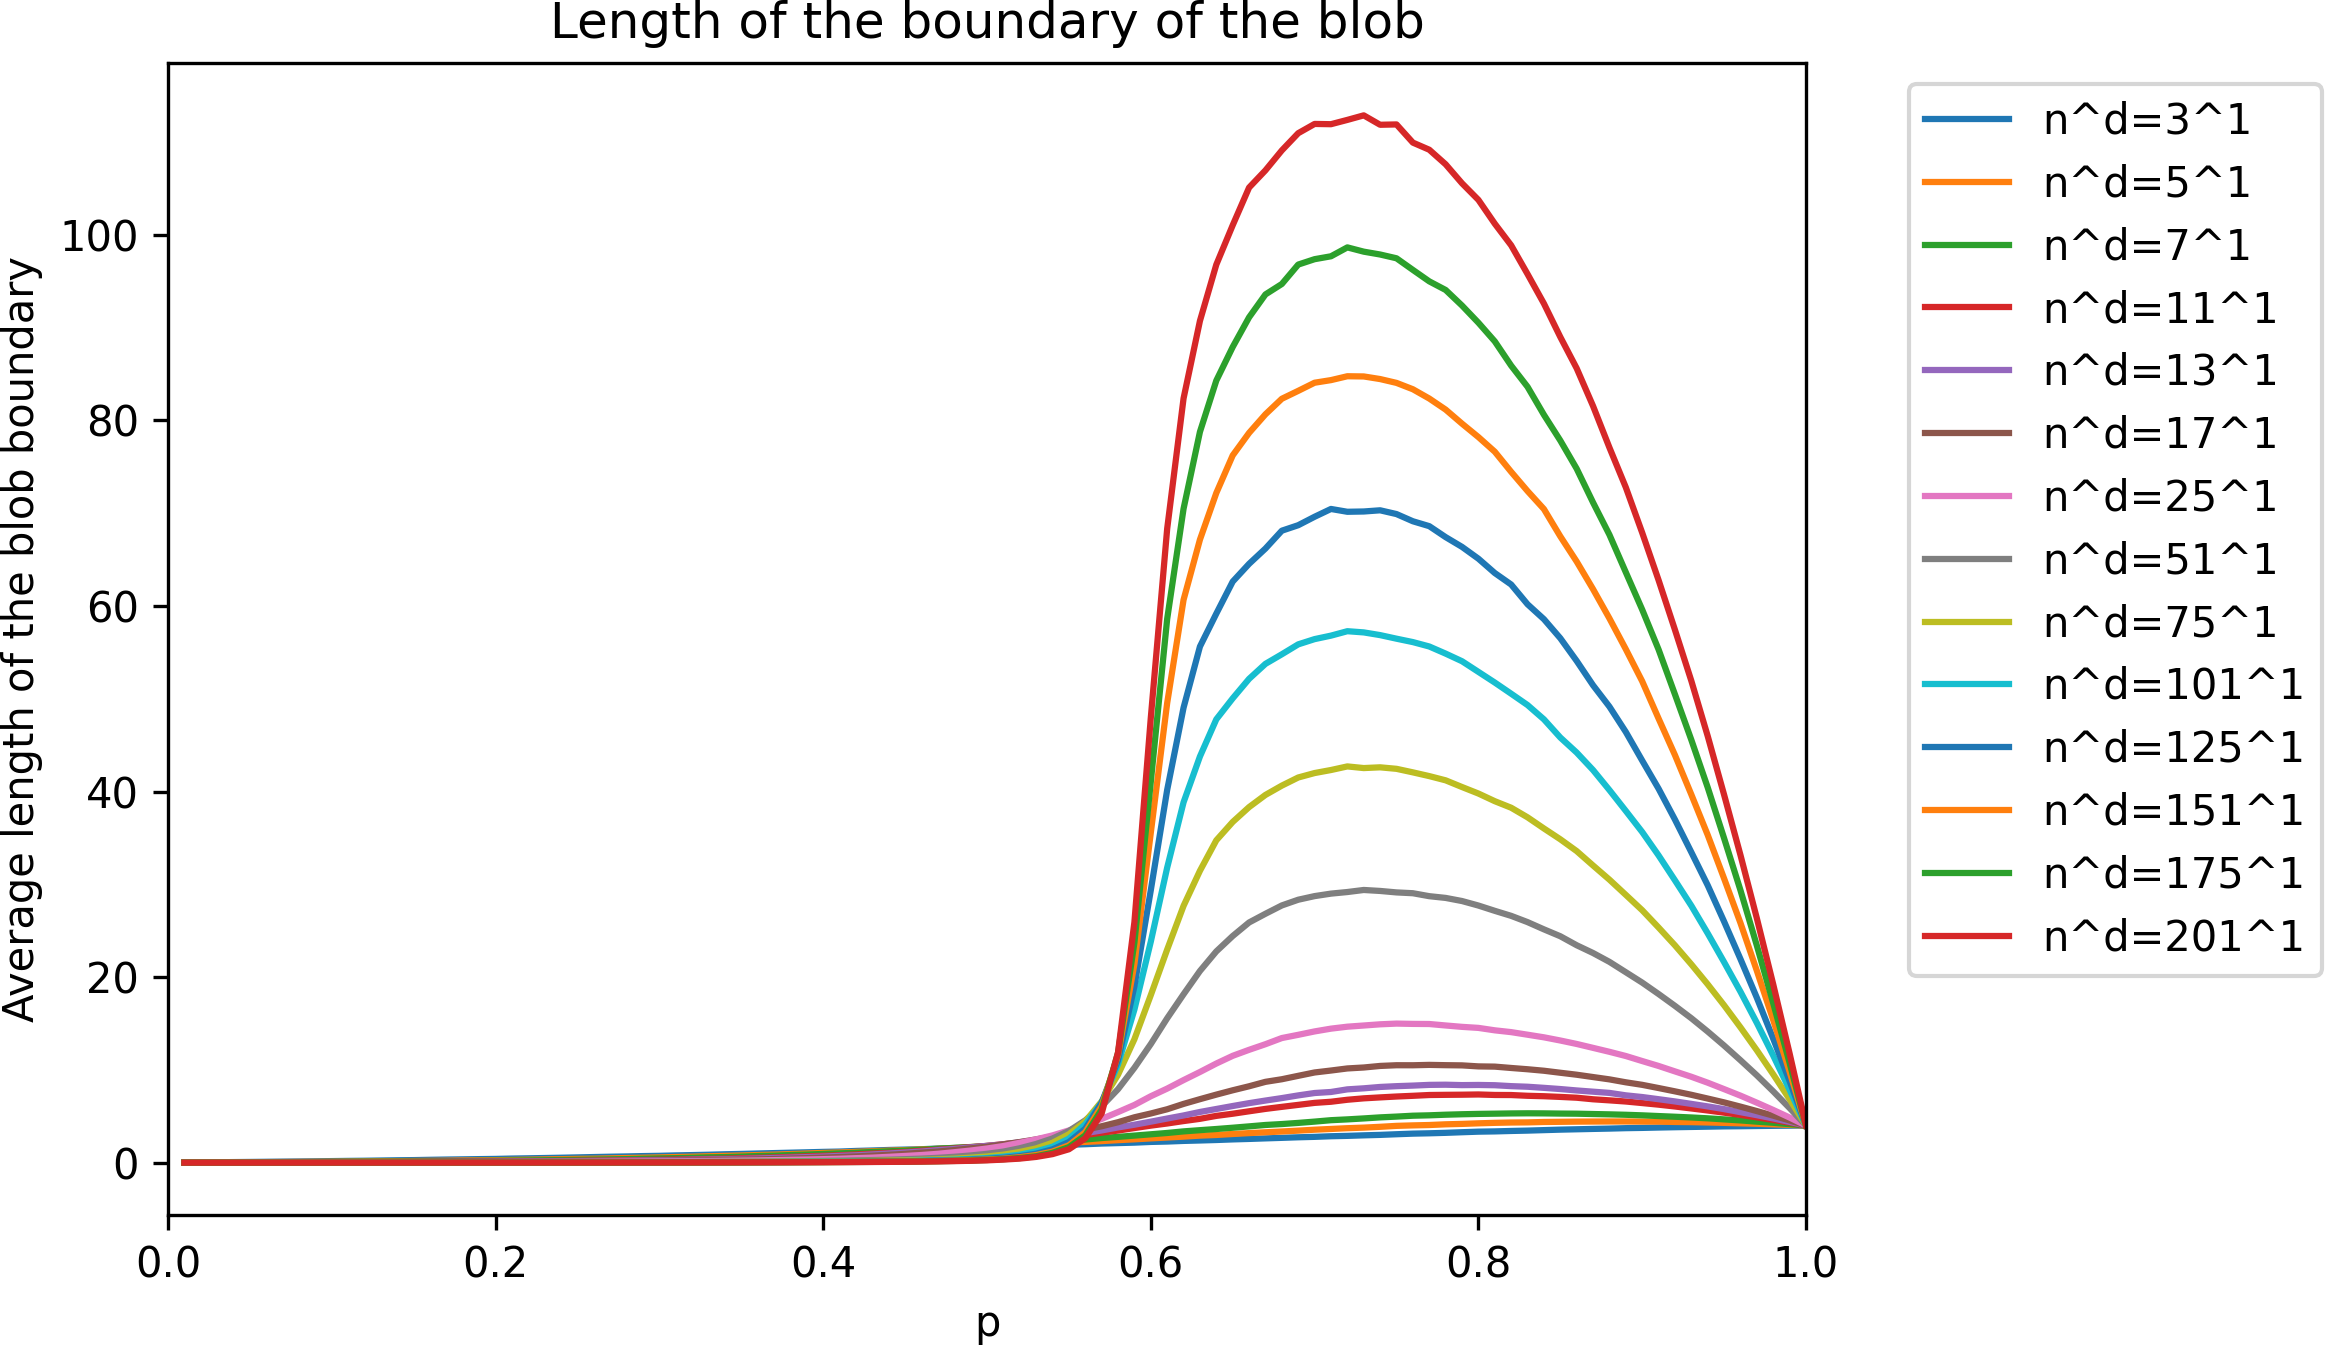
\includegraphics[width=8cm]{blob_boundary_2D_classical}
		\centering
		\caption{Classical Percolation}
		\label{fig:blobBoundaryClassical}
	\end{subfigure}
	\begin{subfigure}{.49\textwidth}
		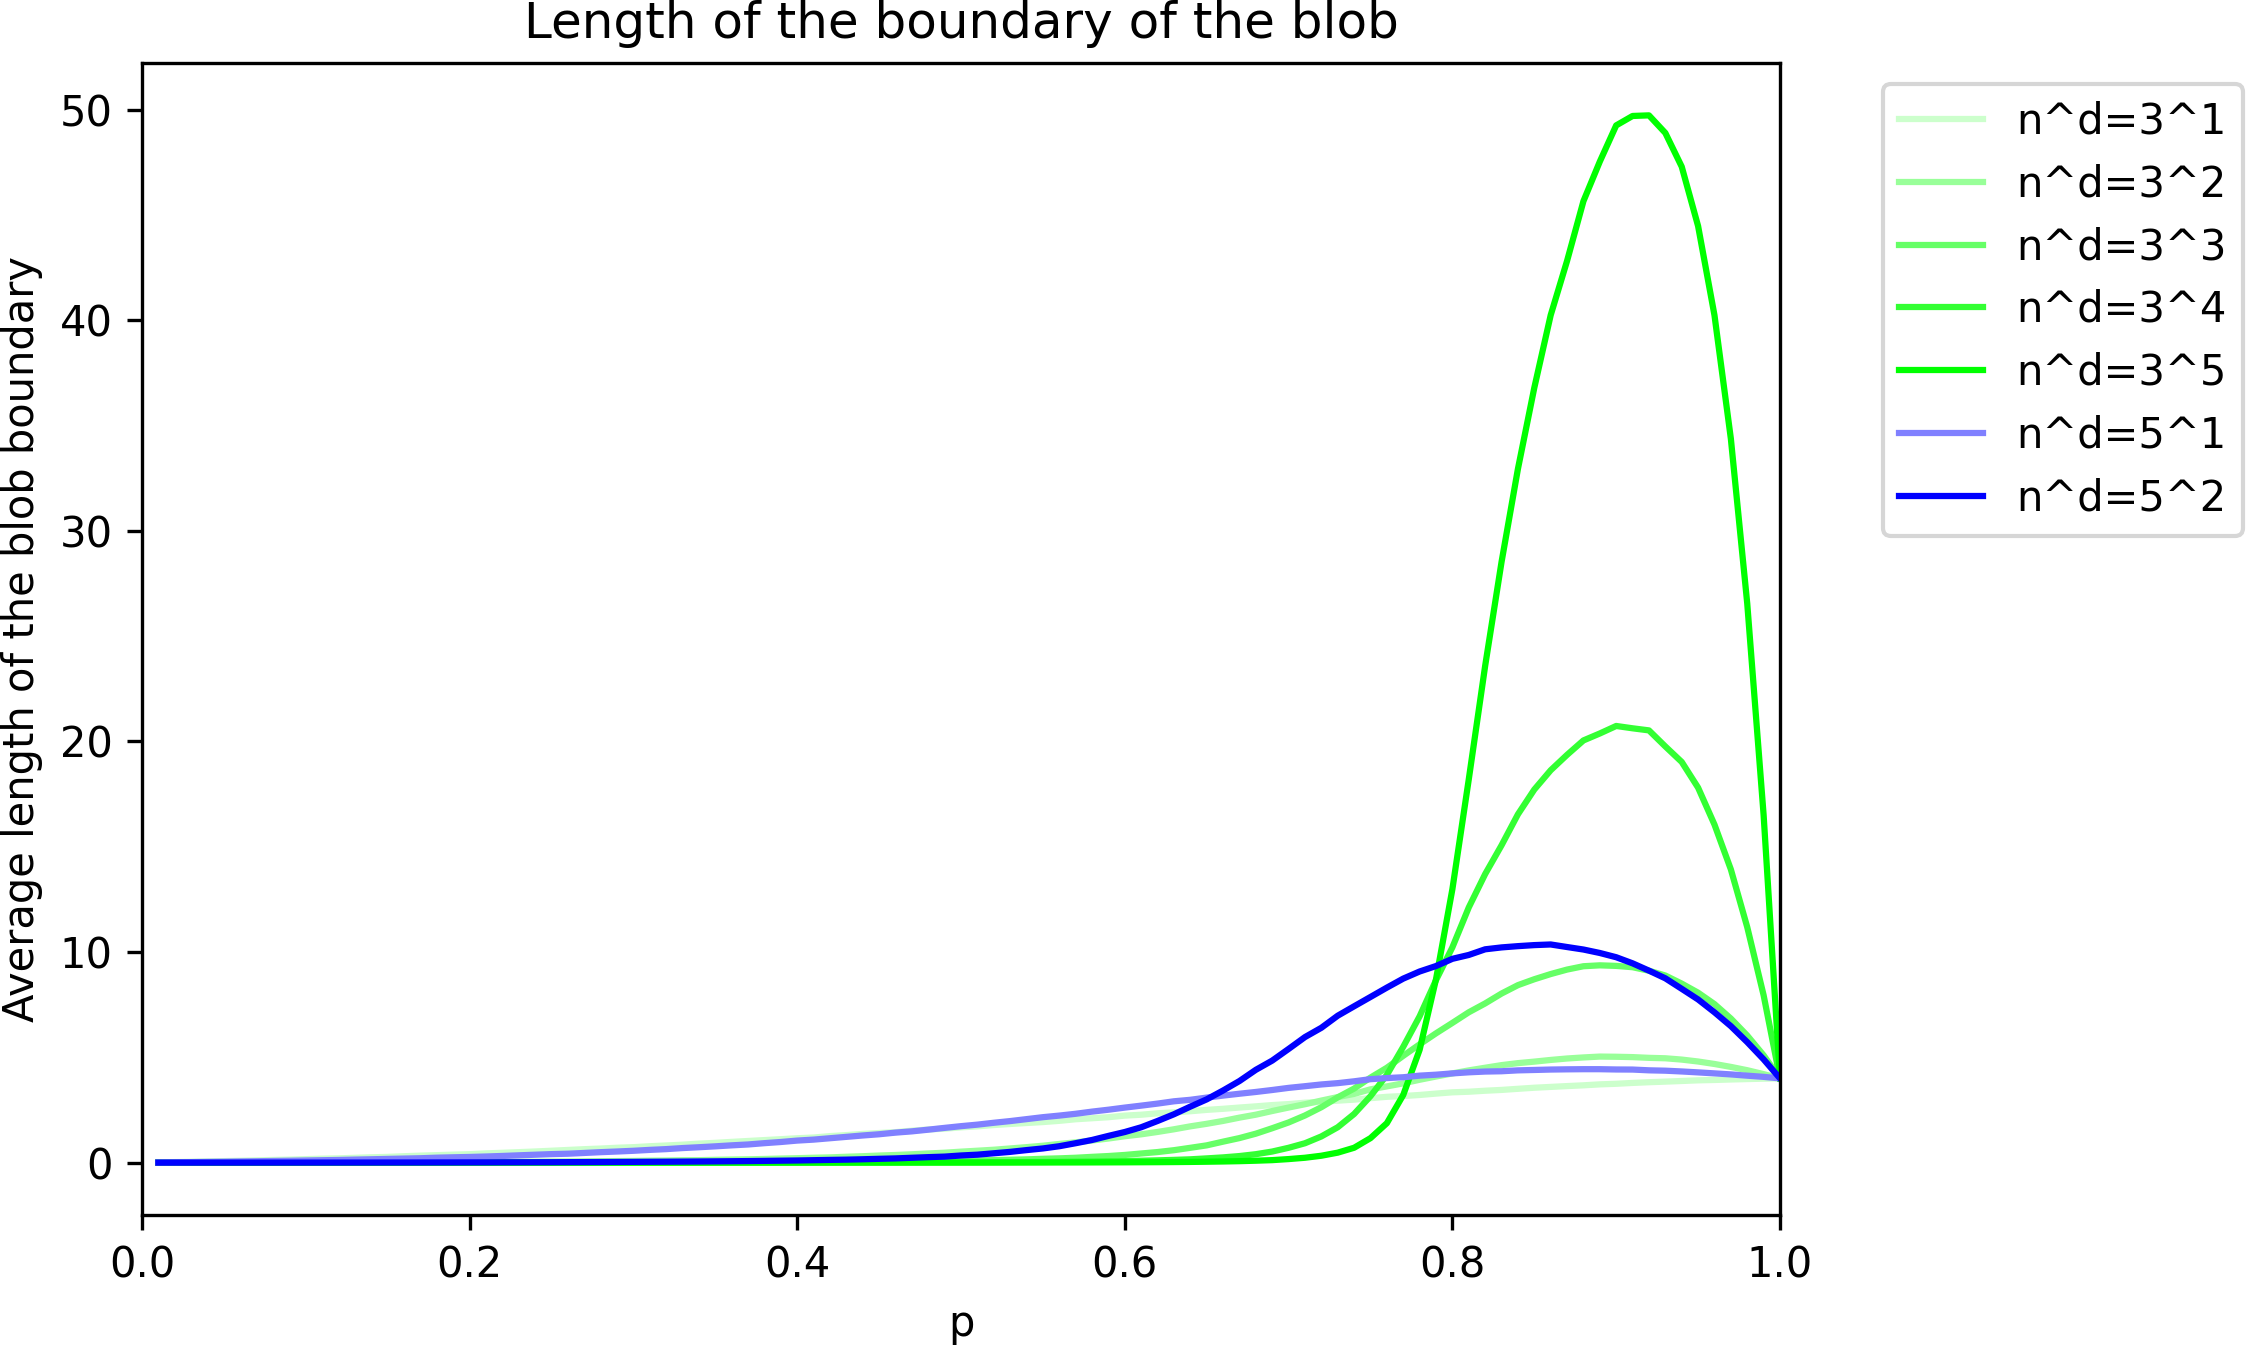
\includegraphics[width=8cm]{blob_boundary_2D_recursive}
		\centering
		\caption{Recursive Percolation}
		\label{fig:blobBoundaryRecursive}
	\end{subfigure}
	\caption{Blob Boundary}
	\label{fig:blobBoundary}
\end{figure}


\subparagraph{Step distance center-border}
The step distance measures a mix of the blob size and its irregularity: a large blob will need many steps to link the center to its boundary (in a similar way to Euclidean distance); and an irregular blob will need a lot of steps to link the center to the boundary, as the path will need to labyrinth round the blob's holes.

For this reason, from fig. \ref{fig:blobStepDistanceClassical}, we can extrapolate that as $n \to \infty$, there are two peaks: the first at $p \approx 0.6$ corresponding to the point where the blob stops being nearly empty most times, but the blob is still irregular, resulting in a large center to border step distance; the second at $p = 1$, when the blob is almost the full unit cuboid resulting in a step distance of $1$.
In between, the step distance drops as the blob is neither very large, nor very irregular.

On fig. \ref{fig:blobStepDistanceRecursive}, the step distance collapses as $d \to \infty$.
This is explained by the fact that the percolation density goes to zero, so the blob is empty in most cases.
Thus, the step distance is nearly zero on average.

\begin{figure}[!h]
	\centering
	\begin{subfigure}{.49\textwidth}
		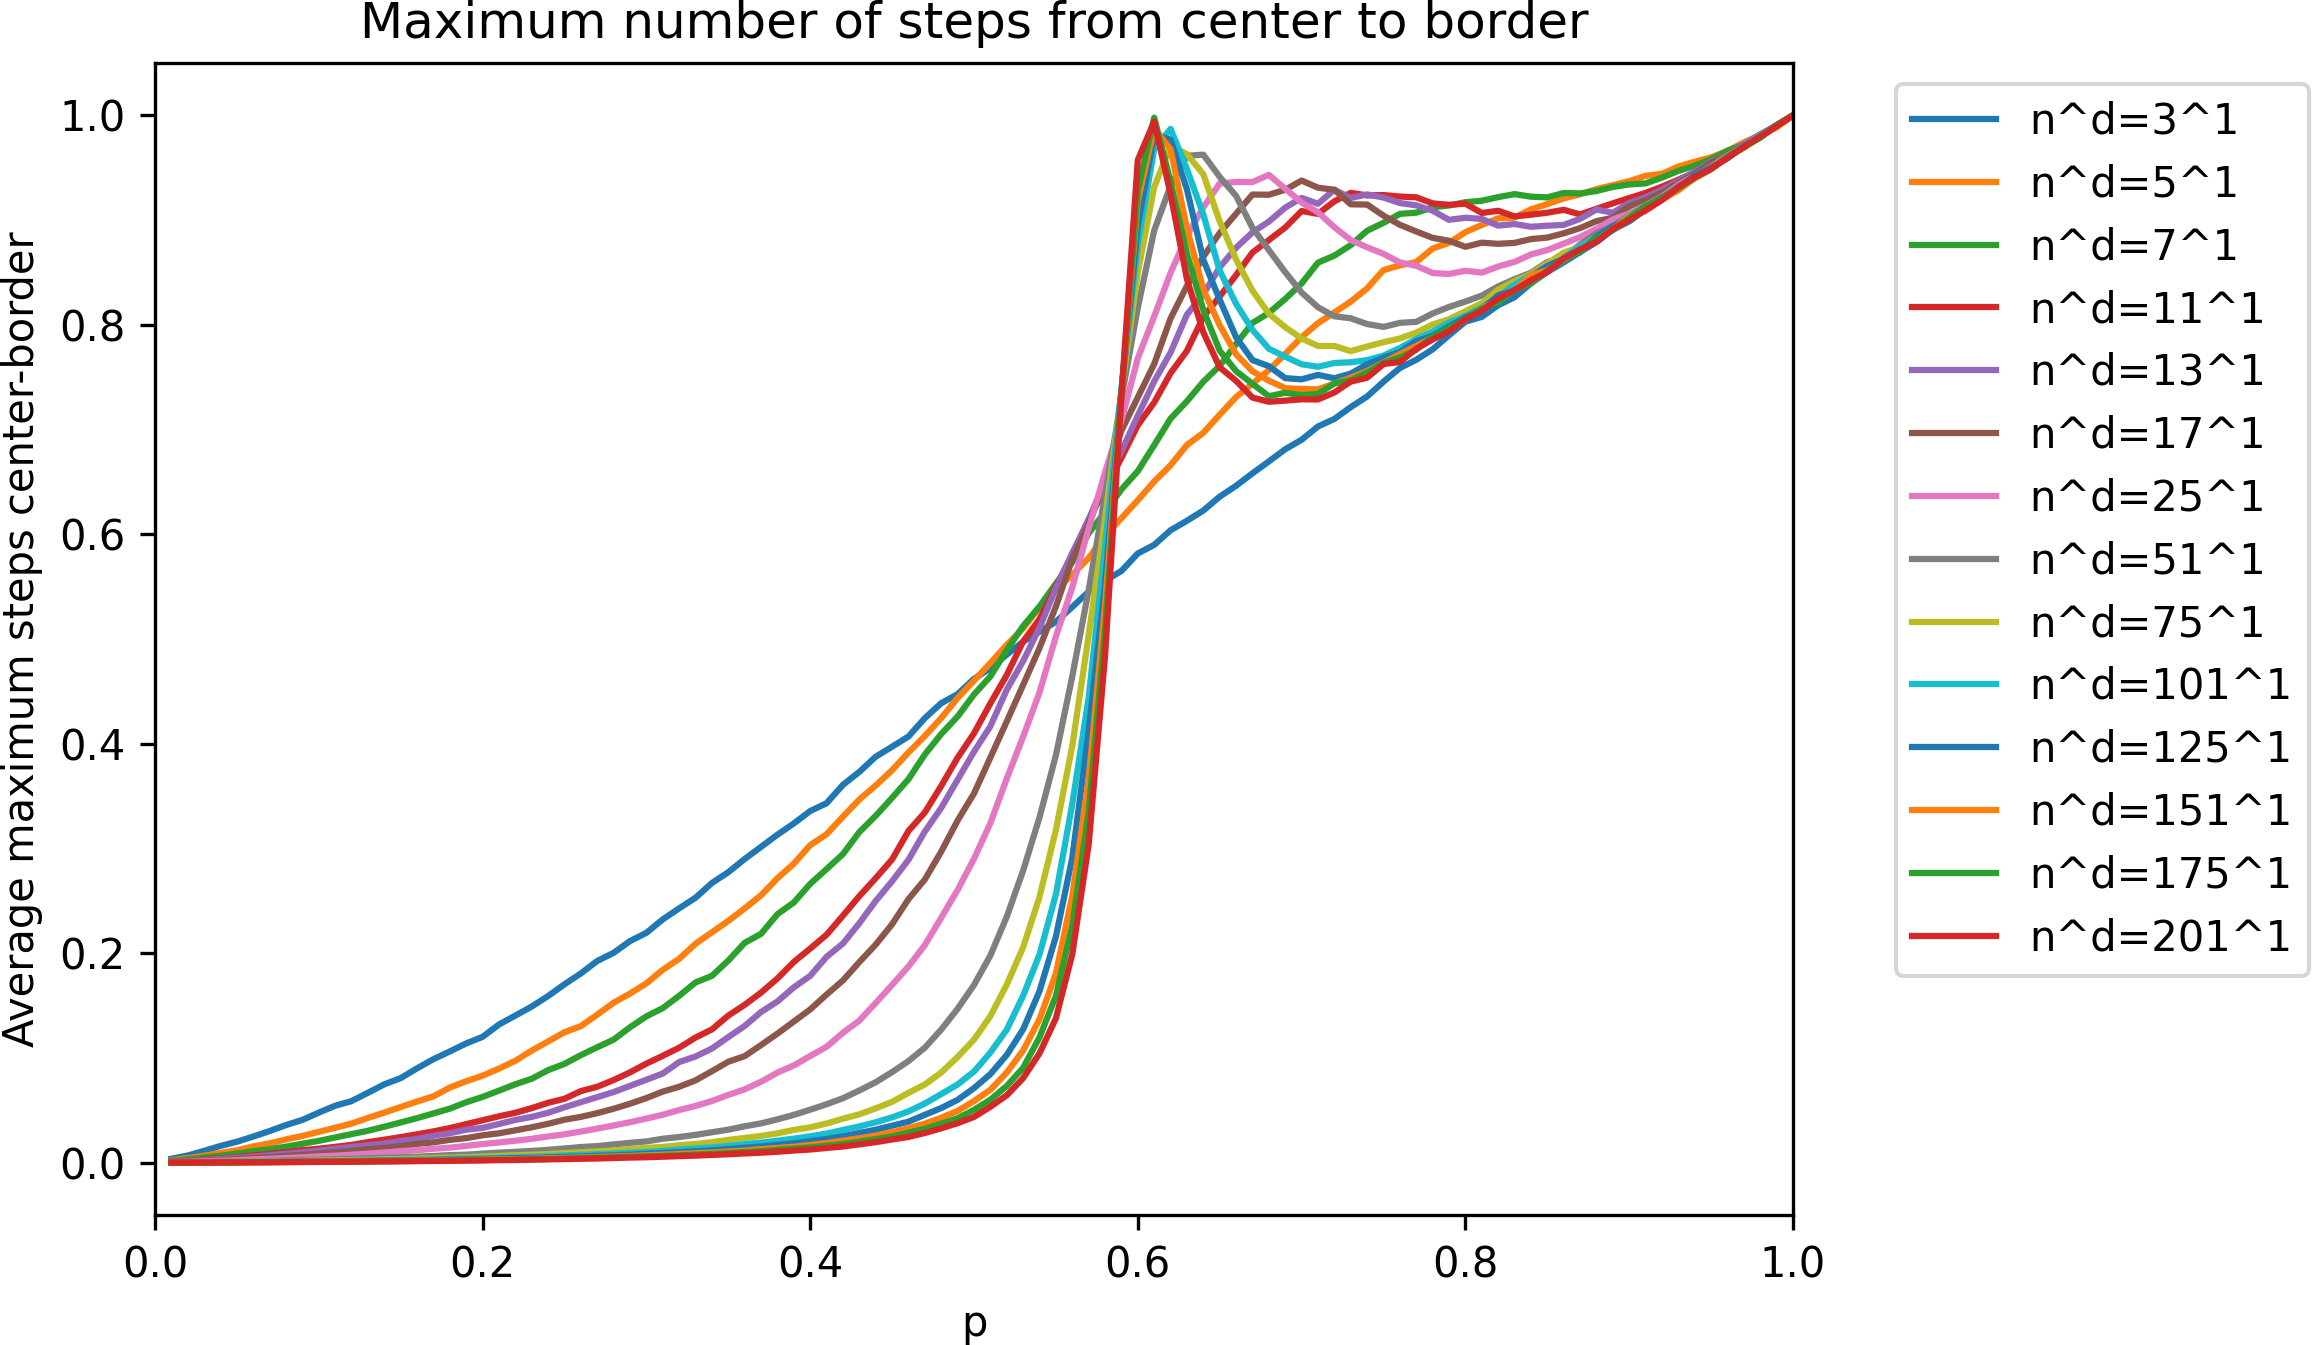
\includegraphics[width=8cm]{blob_step_2D_classical}
		\centering
		\caption{Classical Percolation}
		\label{fig:blobStepDistanceClassical}
	\end{subfigure}
	\begin{subfigure}{.49\textwidth}
		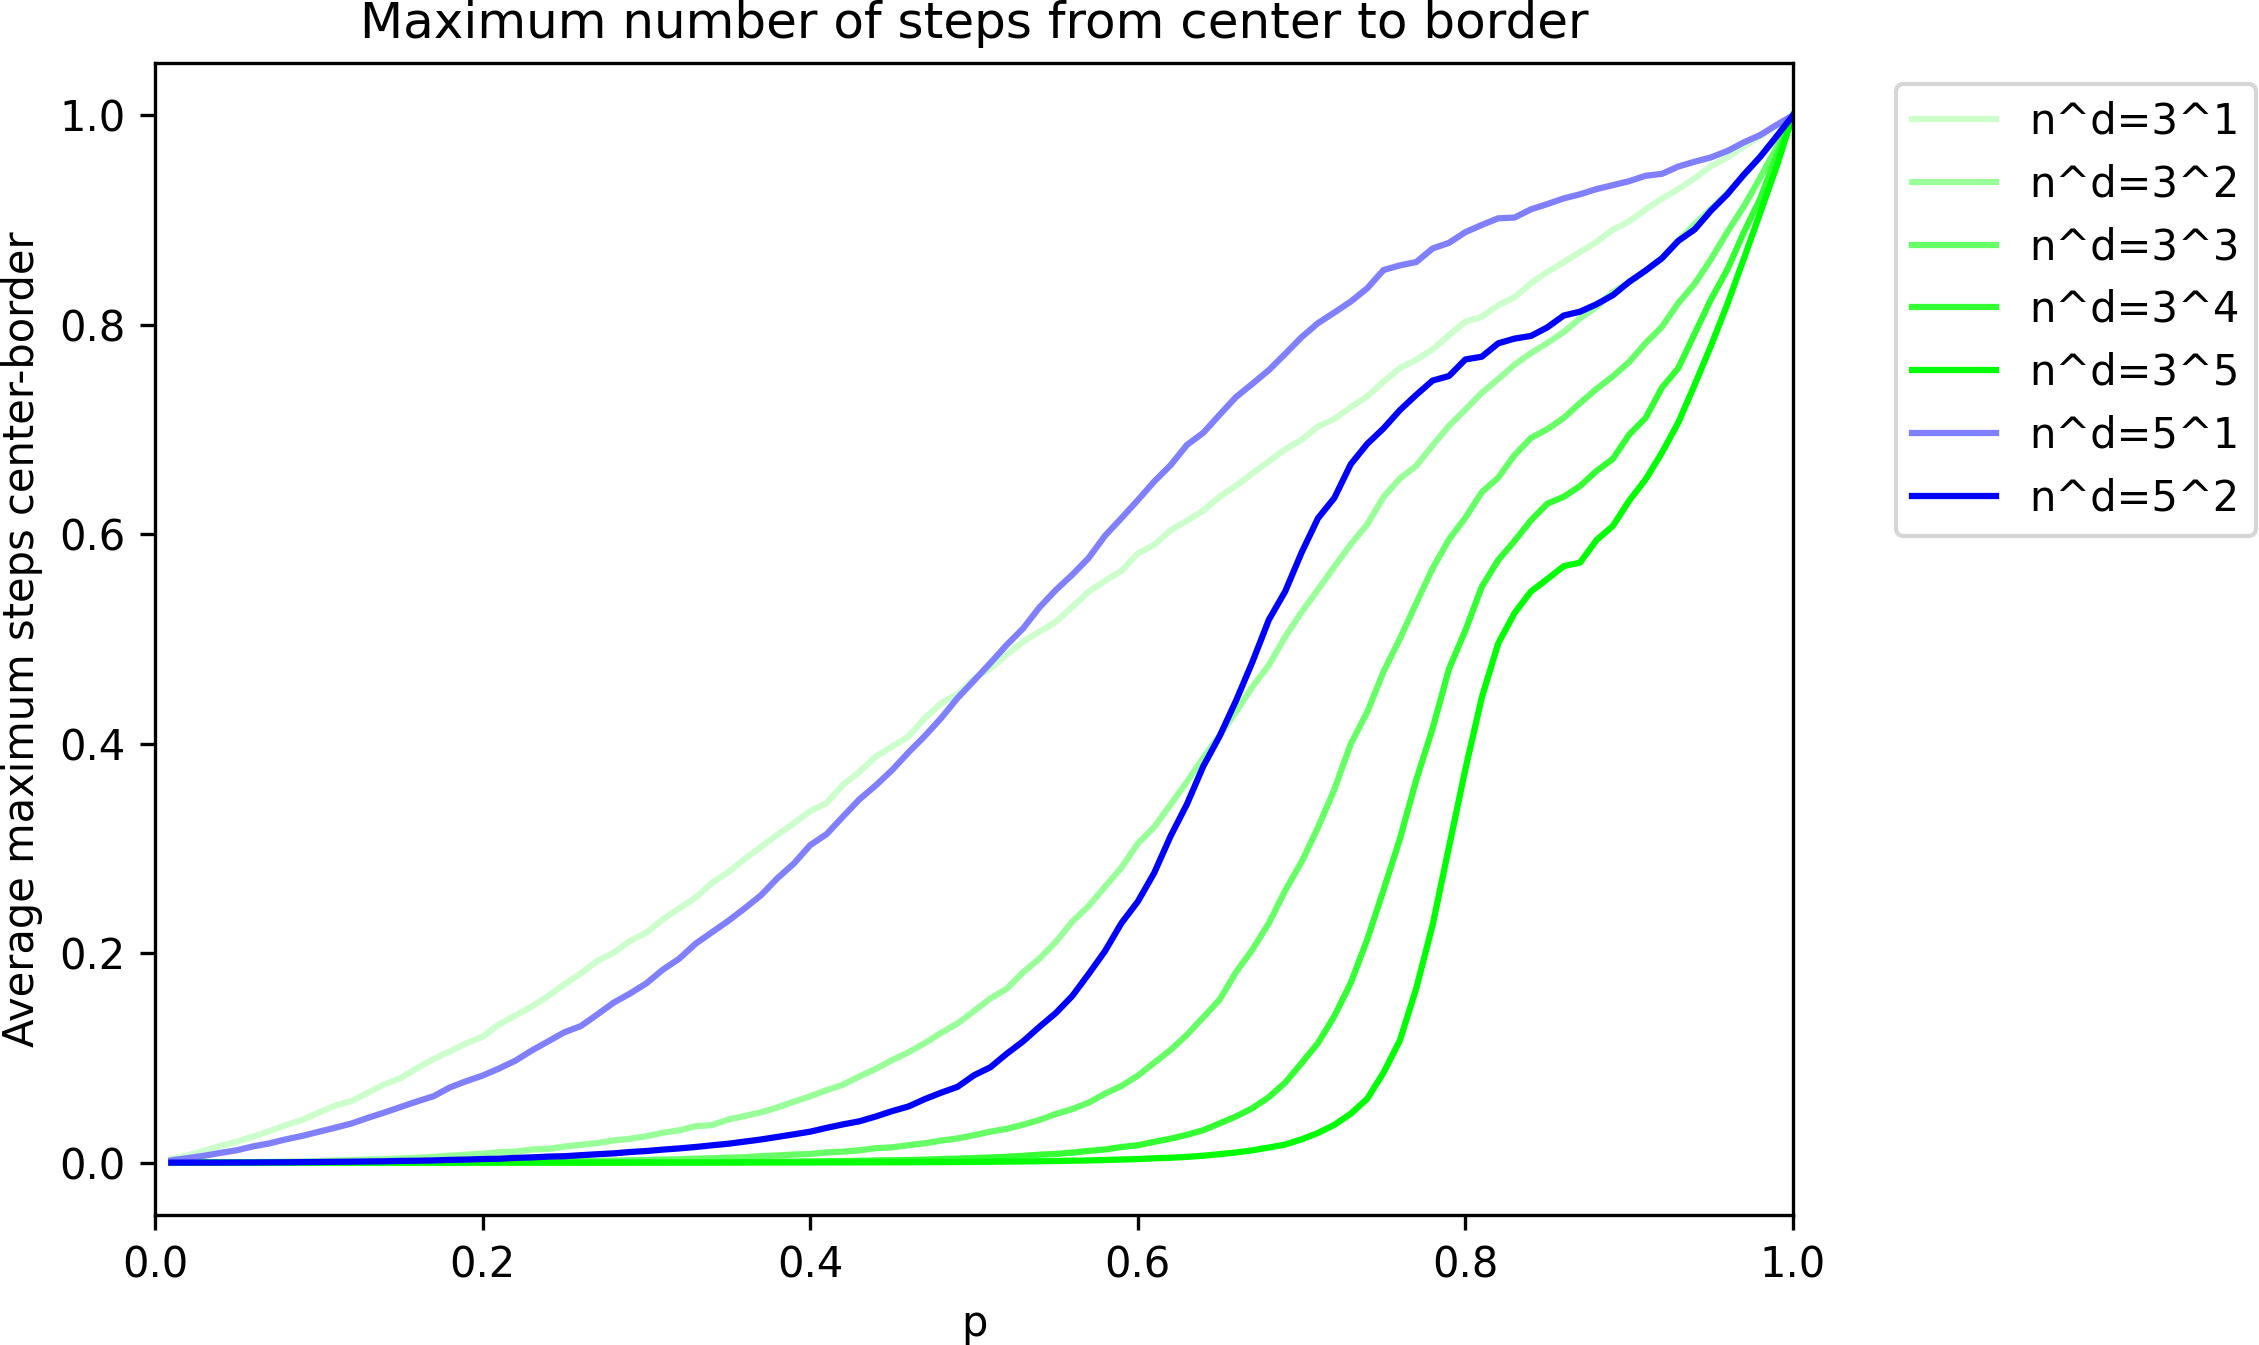
\includegraphics[width=8cm]{blob_step_2D_recursive}
		\centering
		\caption{Recursive Percolation}
		\label{fig:blobStepDistanceRecursive}
	\end{subfigure}
	\caption{Blob Step Distance}
	\label{fig:blobStepDistance}
\end{figure}

%\subsection{Random Walks}

